% =============================================================================
% StockSense AI — VIT-AP University BTech SDP Report
% Author : Vyshakh Vijayan (22BCB7055)
% Branch : Computer Science and Business Systems
% Guide  : Dr. / Mr. / Ms. [GUIDE NAME] — fill before submission
% Date   : May 2025
% Compile: pdflatex -> bibtex -> pdflatex -> pdflatex  (or use Overleaf)
% =============================================================================

\documentclass[12pt,a4paper,oneside]{report}

% ── Core packages ─────────────────────────────────────────────────────────────
\usepackage[
  left   = 3.81cm,
  right  = 2.54cm,
  top    = 2.54cm,
  bottom = 2.54cm
]{geometry}

\usepackage{times}          % Times New Roman
\usepackage[T1]{fontenc}
\usepackage[utf8]{inputenc}
\usepackage{setspace}       % line spacing
\usepackage{parskip}        % paragraph spacing
\usepackage{titlesec}       % heading styles
\usepackage{titletoc}       % TOC styles
\usepackage{fancyhdr}       % headers/footers
\usepackage{emptypage}      % suppress headers on blank pages
\usepackage{graphicx}
\usepackage{float}
\usepackage{caption}
\usepackage{booktabs}
\usepackage{tabularx}
\usepackage{longtable}
\usepackage{array}
\usepackage{multirow}
\usepackage{amsmath}
\usepackage{amssymb}
\usepackage{xcolor}
\usepackage{enumitem}
% \usepackage{microtype}      % disabled — slow on Overleaf free plan
\usepackage{etoolbox}
\usepackage{appendix}
\usepackage{listings}
\usepackage{tikz}
% pgf-umlsd removed — not used in this report
\usepackage[hidelinks]{hyperref}
\usepackage{url}
\usepackage{tfrupee}

\usetikzlibrary{shapes.geometric,arrows.meta,positioning,calc,fit,backgrounds,decorations.pathreplacing}
\usetikzlibrary{external}
\tikzexternalize[prefix=tikz-cache/]

% ── Caption font (min 10pt) ───────────────────────────────────────────────────
\captionsetup{font=small, labelfont=bf, skip=6pt}

% ── Body: 1.5 spacing ─────────────────────────────────────────────────────────
\onehalfspacing

% ── No paragraph indent; small gap between paragraphs ─────────────────────────
\setlength{\parindent}{0pt}
\setlength{\parskip}{6pt}

% ── Chapter heading: Centered, Chapter N (12pt), Title (16pt) ─────────────────
\titleformat{\chapter}[display]
  {\normalfont\centering}
  {\fontsize{12}{16}\bfseries Chapter \thechapter}
  {6pt}
  {\fontsize{16}{20}\bfseries}
\titlespacing*{\chapter}{0pt}{-20pt}{18pt}

% ── Section heading: 14pt CAPS ───────────────────────────────────────────────
\titleformat{\section}
  {\normalfont\fontsize{14}{18}\bfseries\MakeUppercase}
  {\thesection}
  {1em}
  {}
\titlespacing*{\section}{0pt}{14pt}{6pt}

% ── Subsection heading: 12pt CAPS ────────────────────────────────────────────
\titleformat{\subsection}
  {\normalfont\fontsize{12}{16}\bfseries\MakeUppercase}
  {\thesubsection}
  {1em}
  {}
\titlespacing*{\subsection}{0pt}{12pt}{4pt}

% ── Subsubsection heading: 12pt Bold (normal case) ───────────────────────────
\titleformat{\subsubsection}
  {\normalfont\fontsize{12}{16}\bfseries}
  {\thesubsubsection}
  {1em}
  {}

% ── Page style: bottom-centre page numbers ────────────────────────────────────
\fancypagestyle{mainpages}{%
  \fancyhf{}
  \renewcommand{\headrulewidth}{0pt}
  \fancyfoot[C]{\thepage}
}
\fancypagestyle{plain}{%
  \fancyhf{}
  \renewcommand{\headrulewidth}{0pt}
  \fancyfoot[C]{\thepage}
}
\pagestyle{mainpages}

% ── Widow / orphan control ────────────────────────────────────────────────────
\widowpenalty=10000
\clubpenalty=10000

% ── Listings configuration ───────────────────────────────────────────────────
\lstdefinelanguage{javascript}{
  keywords={break, case, catch, continue, debugger, default, delete, do, else, false, finally, for, function, if, in, instanceof, new, null, return, switch, this, throw, true, try, typeof, var, void, while, with, let, const, async, await, export, import, from},
  morecomment=[l]{//},
  morecomment=[s]{/*}{*/},
  morestring=[b]',
  morestring=[b]",
  ndkeywords={class, export, boolean, throw, implements, import, this},
  sensitive=true
}

\lstset{
  basicstyle=\footnotesize\ttfamily,
  breaklines=true,
  breakatwhitespace=true,
  numbers=left,
  numberstyle=\tiny,
  numbersep=5pt,
  frame=single,
  tabsize=2,
  showstringspaces=false,
  keywordstyle=\bfseries\color{blue},
  commentstyle=\itshape\color{gray!60},
  stringstyle=\color{green!50!black},
  extendedchars=true,
  literate={Rs.}{{Rs.}}2 {á}{{\'a}}1 {é}{{\'e}}1 {í}{{\'i}}1 {ó}{{\'o}}1 {ú}{{\'u}}1,
}

% ── TikZ workflow node styles ─────────────────────────────────────────────────
\tikzset{
  wfnode/.style={
    rectangle, rounded corners=3pt, draw=black!70, fill=gray!8,
    text width=1.6cm, minimum height=0.75cm,
    align=center, font=\sffamily\scriptsize, inner sep=3pt
  },
  wftrigger/.style={wfnode, fill=gray!22, font=\sffamily\scriptsize\bfseries},
  wfdecision/.style={
    diamond, draw=black!70, fill=gray!8,
    text width=0.9cm, minimum height=0.7cm,
    align=center, font=\sffamily\scriptsize, inner sep=1pt, aspect=2.2
  },
  wfarrow/.style={-Stealth, thick, draw=black!70},
  wflabel/.style={font=\sffamily\tiny, fill=white, inner sep=1pt},
}

% ── Hyperref metadata ─────────────────────────────────────────────────────────
\hypersetup{
  pdftitle  = {StockSense AI: AI-Powered Supply Chain Inventory Intelligence System},
  pdfauthor = {Vyshakh Vijayan},
  colorlinks= false,
  pdfborder = {0 0 0},
}

% =============================================================================
\begin{document}
\sloppy  % globally fix ALL overfull \hbox warnings
% =============================================================================

% ── Front matter (roman numerals) ────────────────────────────────────────────
\pagenumbering{roman}

% =============================================================================
% TITLE PAGE — VIT-AP SDP standard format
% =============================================================================
\begin{titlepage}
\centering

\vspace*{0.5cm}

{\fontsize{12}{14}\selectfont\itshape A project report on}

\vfill

{\fontsize{20}{24}\selectfont\bfseries\MakeUppercase{%
StockSense AI:\\[6pt]
AI-Powered Supply Chain\\[6pt]
Inventory Intelligence System}}

\vfill

{\fontsize{14}{17}\selectfont\itshape
Submitted in partial fulfillment for the award of the degree of}

\vfill

{\fontsize{22}{26}\selectfont\bfseries
Bachelor of Technology in\\[6pt]
Computer Science and Business Systems}

\vfill

{\fontsize{14}{17}\selectfont\itshape by}

\vfill

{\fontsize{16}{20}\selectfont\bfseries\MakeUppercase{Vyshakh Vijayan (22BCB7055)}}

\vfill


\includegraphics[width=9cm]{images/vit_logo.png}

\vfill

{\fontsize{16}{20}\selectfont\bfseries\MakeUppercase{%
School of Computer Science and Engineering}}

\vfill

{\fontsize{12}{14}\selectfont May 2025}

\vspace*{0.5cm}

\end{titlepage}
\clearpage

% =============================================================================
% DECLARATION PAGE
% =============================================================================
\chapter*{DECLARATION}
\addcontentsline{toc}{chapter}{Declaration}
{\centering\fontsize{14}{18}\bfseries\underline{DECLARATION}\par}
\vspace{1cm}

I hereby declare that the thesis entitled \textit{``StockSense AI: AI-Powered Supply Chain
Inventory Intelligence System''} submitted by me, for the award of the degree of Bachelor of
Technology in Computer Science and Business Systems, VIT-AP University is a record of bonafide
work carried out by me under the supervision of Dr.\ [Guide Full Name]. I further declare that the
work reported in this thesis has not been submitted and will not be submitted, either in part or in
full, for the award of any other degree or diploma in this institute or any other institute or
university.

\vspace{3cm}

\noindent
\begin{tabular}{@{}p{0.45\textwidth}@{\hspace{0.1\textwidth}}p{0.45\textwidth}@{}}
\textbf{Place:} Amaravati & \textbf{Signature of the Candidate} \\[0.8cm]
\textbf{Date:} \underline{\hspace{3cm}} & \textbf{Vyshakh Vijayan} \\
 & \textbf{22BCB7055} \\
\end{tabular}

\clearpage

% =============================================================================
% CERTIFICATE PAGE
% =============================================================================
\chapter*{CERTIFICATE}
\addcontentsline{toc}{chapter}{Certificate}
{\centering\fontsize{14}{18}\bfseries\underline{CERTIFICATE}\par}
\vspace{1cm}

This is to certify that the Senior Design Project titled \textit{``StockSense AI: AI-Powered
Supply Chain Inventory Intelligence System''} that is being submitted by \textbf{Vyshakh Vijayan
(22BCB7055)} is in partial fulfillment of the requirements for the award of Bachelor of Technology
in Computer Science and Business Systems, is a record of bonafide work done under my guidance.
The contents of this Project work, in full or in parts, have neither been taken from any other
source nor have been submitted to any other Institute or University for award of any degree or
diploma and the same is certified.

\vspace{3.5cm}

\noindent
\begin{tabular}{@{}p{0.45\textwidth}@{\hspace{0.1\textwidth}}p{0.45\textwidth}@{}}
\textbf{Internal Guide} & \textbf{Internal Examiner} \\[0.4cm]
Dr.\ [Guide Full Name] & [Examiner Name] \\
[Designation] & [Designation] \\
School of CSE, VIT-AP & School of CSE, VIT-AP \\[2.0cm]

\textbf{External Examiner} & \textbf{Dean} \\[0.4cm]
[External Examiner Name] & [Dean Name] \\
[Designation \& Institution] & School of Computer Science and Engineering \\
 & VIT-AP University, Amaravati \\
\end{tabular}

\vspace{1.5cm}

\noindent
\textbf{Place:} Amaravati \hspace{2cm} \textbf{Date:} \underline{\hspace{3cm}}

\clearpage

% =============================================================================
% ABSTRACT  (roman page i)
% =============================================================================
\chapter*{ABSTRACT}
\addcontentsline{toc}{chapter}{Abstract}
{\centering\fontsize{14}{18}\bfseries\underline{ABSTRACT}\par}
\vspace{0.8cm}

Inventory mismanagement is one of the most persistent operational challenges confronting small-scale
retail outlets in India, commonly referred to as kirana stores. These establishments, numbering
approximately twelve million across the country, continue to rely on manual record-keeping methods
such as physical ledgers or basic spreadsheet tools, which are ill-suited for real-time stock
monitoring, demand forecasting, or supplier evaluation. Enterprise-grade solutions designed for
large retail chains are financially prohibitive and operationally complex for single-owner
businesses that typically lack dedicated information technology personnel.

In response to this gap, a system named StockSense AI was designed and developed as an
intelligent, low-cost inventory management solution tailored specifically to the operational
context of small Indian retailers. The proposed system integrates automated workflow orchestration,
artificial intelligence-driven decision support, and real-time communication into a cohesive
platform that requires minimal technical expertise to operate.

The architecture of StockSense AI consists of four principal layers: a React~19 single-page
application serving as the user-facing frontend, an n8n-based workflow automation engine
comprising ten modular workflows constituting the backend intelligence pipeline, a Supabase
PostgreSQL database providing persistent storage and real-time data propagation, and an external
services layer incorporating the Groq Llama~3.1~8B large language model, Google Gemini~2.5
Flash multimodal model, and Twilio WhatsApp Business API.

The system automates stockout date prediction through a sales-velocity formula, classifies
products into risk tiers, generates natural-language reorder suggestions with supplier-level
reasoning, scores suppliers using a multi-criteria Weighted Sum Model, and delivers formatted
stock alerts directly to the store owner's WhatsApp account. An AI vision module enables
product onboarding from a photograph, while a separate invoice scanning workflow automates
stock-level updates from supplier delivery bills.

The prototype was evaluated against a dataset of ten products and four suppliers across multiple
inventory states. The complete intelligence pipeline executes in approximately thirteen seconds,
WhatsApp message delivery is achieved within five seconds of pipeline completion, and the
total infrastructure cost for production deployment remains below five hundred rupees per month.
The system thus demonstrates that advanced inventory intelligence, previously accessible only to
large retail enterprises, can be delivered to kirana store owners at a practically negligible cost.

\vspace{0.8cm}
\noindent\textbf{Keywords:} Inventory Management, Supply Chain Intelligence, Workflow Automation,
n8n, Large Language Model, Supplier Scoring, Kirana Stores, SME Technology, Stockout Prediction,
WhatsApp Alerts.

\clearpage

% =============================================================================
% ACKNOWLEDGEMENT  (roman page ii)
% =============================================================================
\chapter*{ACKNOWLEDGEMENT}
\addcontentsline{toc}{chapter}{Acknowledgement}
{\centering\fontsize{14}{18}\bfseries\underline{ACKNOWLEDGEMENT}\par}
\vspace{0.8cm}

I express my sincere and heartfelt gratitude to my project guide, \textbf{Dr.\ [Guide Full Name]},
[Designation], School of Computer Science and Engineering, VIT-AP University, for the continuous
support, invaluable guidance, and scholarly encouragement extended throughout the course of this
Senior Design Project. The technical insights and constructive feedback provided by my guide played
a pivotal role in shaping both the conceptual foundation and the practical implementation of
StockSense AI.

I am deeply indebted to the distinguished leadership of VIT-AP University — the Chancellor,
Vice-President, Vice-Chancellor, and the Dean of the School of Computer Science and Engineering —
for fostering a vibrant academic environment that consistently encourages student-driven innovation.
The infrastructure, resources, and intellectual culture made available by the institution have
been fundamental to the successful completion of this project.

I extend my appreciation to the Program Chair and the entire faculty of the School of Computer
Science and Engineering for their academic mentorship over the course of the undergraduate program.
Their guidance in developing a strong foundation in both theoretical concepts and practical
engineering principles has been instrumental in enabling this work.

I am profoundly grateful to my parents and family members for their unconditional support,
patience, and encouragement throughout my academic journey. Their sacrifices and constant
motivation have been the driving force behind every milestone achieved.

Finally, I wish to thank my friends and classmates for their encouragement, stimulating
discussions, and camaraderie. The collaborative spirit within the cohort made the demanding
process of research and development considerably more rewarding.

\vspace{2.5cm}

\noindent
\begin{tabular}{@{}p{0.45\textwidth}@{\hspace{0.1\textwidth}}p{0.45\textwidth}@{}}
\textbf{Place:} Amaravati & \\[0.5cm]
\textbf{Date:} \underline{\hspace{3cm}} & \textbf{Vyshakh Vijayan} \\
 & \textbf{22BCB7055} \\
\end{tabular}

\clearpage


% ── TOC / LOF / LOT / Abbreviations ─────────────────────────────────────────
{
  \singlespacing
  \setcounter{tocdepth}{3}
  \tableofcontents
  \clearpage
  \listoffigures
  \clearpage
  \listoftables
  \clearpage
}
% =============================================================================
% LIST OF ABBREVIATIONS
% =============================================================================
\chapter*{LIST OF ABBREVIATIONS}
\addcontentsline{toc}{chapter}{List of Abbreviations}
{\centering\fontsize{14}{18}\bfseries\underline{LIST OF ABBREVIATIONS}\par}
\vspace{0.8cm}

{\singlespacing
\begin{longtable}{@{}p{0.25\textwidth} p{0.70\textwidth}@{}}
\toprule
\textbf{Abbreviation} & \textbf{Full Form} \\
\midrule
\endhead
AI      & Artificial Intelligence \\
API     & Application Programming Interface \\
CORS    & Cross-Origin Resource Sharing \\
CRUD    & Create, Read, Update, Delete \\
CSV     & Comma-Separated Values \\
CSS     & Cascading Style Sheets \\
DB      & Database \\
ERP     & Enterprise Resource Planning \\
FAQ     & Frequently Asked Questions \\
FK      & Foreign Key \\
HTTP    & Hypertext Transfer Protocol \\
HTTPS   & Hypertext Transfer Protocol Secure \\
ID      & Identifier \\
IoT     & Internet of Things \\
IST     & Indian Standard Time \\
JSON    & JavaScript Object Notation \\
JWT     & JSON Web Token \\
KPI     & Key Performance Indicator \\
LLM     & Large Language Model \\
LOF     & List of Figures \\
LOT     & List of Tables \\
ML      & Machine Learning \\
MSME    & Micro, Small and Medium Enterprises \\
n8n     & Node-based workflow automation platform \\
OOS     & Out of Stock \\
PK      & Primary Key \\
POS     & Point of Sale \\
REST    & Representational State Transfer \\
RFID    & Radio Frequency Identification \\
RLS     & Row Level Security \\
SaaS    & Software as a Service \\
SDP     & Senior Design Project \\
SME     & Small and Medium Enterprise \\
SPA     & Single-Page Application \\
SQL     & Structured Query Language \\
TOC     & Table of Contents \\
UI      & User Interface \\
UPI     & Unified Payments Interface \\
URL     & Uniform Resource Locator \\
UUID    & Universally Unique Identifier \\
UX      & User Experience \\
VIT-AP  & Vellore Institute of Technology -- Andhra Pradesh \\
WF      & Workflow \\
WSM     & Weighted Sum Model \\
\bottomrule
\end{longtable}
}
\clearpage


% ── Main matter (arabic numerals) ────────────────────────────────────────────
\pagenumbering{arabic}
\setcounter{page}{1}

% =============================================================================
% CHAPTER 1 — INTRODUCTION
% =============================================================================
\chapter{Introduction}
\label{ch:intro}

\section{Introduction}

India's retail sector is anchored by approximately twelve million kirana stores — neighbourhood
grocery and general merchandise outlets that serve as the primary point of purchase for a large
proportion of the country's population. These stores collectively account for over ninety percent
of the food and grocery retail market by volume and represent a cornerstone of India's informal
economy. Despite their economic significance, the vast majority of these establishments continue
to operate without the benefit of any digital inventory management system. Inventory decisions are
typically made on the basis of the owner's intuition, physical counting, or entries in paper
ledgers, practices that are inherently error-prone and incapable of adapting to the dynamic
consumer demand patterns of today's retail environment.

The consequences of this operational gap are commercially significant. A stockout event — where
a product runs out before the next replenishment order arrives — results in a direct loss of
revenue and a deterioration of customer trust. Conversely, overstocking ties up working capital
in slow-moving goods and increases the risk of spoilage for perishable items. Without a
systematic approach to tracking sales velocity, predicting replenishment needs, and evaluating
supplier performance, kirana store owners are left managing these risks entirely through manual
estimation.

Enterprise Resource Planning (ERP) solutions that address these challenges for large retailers
are commercially available but are wholly unsuitable for the kirana store context. Monthly
subscription costs ranging from several thousand to tens of thousands of rupees, complex
onboarding processes, and hardware requirements such as barcode scanners and RFID readers place
these systems well beyond the reach of a typical small store owner. Simpler Point-of-Sale (POS)
applications record transactions but lack the predictive analytics and automated alerting
capabilities necessary to prevent stockout situations proactively.

The emergence of low-code automation platforms, cloud-hosted databases, and large language model
APIs accessible at low or zero cost has created a new opportunity: it is now technically feasible
to build a fully functional, automated inventory intelligence system for a fraction of the cost
of traditional enterprise software. StockSense AI is designed to exploit precisely this
opportunity.

\section{Problem Statement}

Small retail stores in India lack an affordable and automated inventory management system that can predict stockout dates, generate supplier-aware reorder suggestions, score vendors, and deliver alerts through channels like WhatsApp. Existing solutions are financially and operationally inaccessible, while basic tools only provide passive recording without intelligence.

The core problem to be solved is therefore: \textit{How can an automated, AI-augmented inventory
intelligence pipeline be built and deployed for kirana stores at an infrastructure cost below
\rupee{}500 per month, requiring no technical expertise to operate on a day-to-day basis?}

\section{Objectives}

The following specific objectives have been established to guide the design and development of
StockSense AI:

\begin{enumerate}[label=\textbf{\arabic*.}, leftmargin=*, itemsep=4pt]
  \item To design and implement an automated pipeline that calculates stockout dates for all
        inventory items using daily sales velocity and updates product risk classifications
        (HIGH, MEDIUM, LOW) without manual intervention.

  \item To develop an AI reorder recommendation engine using Groq Llama 3.1 8B that generates
        natural-language suggestions with supplier selection reasoning based on stock levels,
        demand patterns, and performance grades.

  \item To build a supplier evaluation module using the Weighted Sum Model (WSM) that assigns
        composite performance scores and letter grades to suppliers based on reliability,
        pricing, and delivery speed criteria.

  \item To implement a real-time WhatsApp alert delivery system using the Twilio API that
        notifies store owners of critical stock conditions immediately upon pipeline execution,
        incorporating a 24-hour anti-spam cooldown mechanism.

  \item To create AI vision-powered features — product onboarding via photograph and supplier
        invoice scanning using Google Gemini~2.5 Flash — that automate data entry and eliminate
        manual stock update procedures.

  \item To deploy the complete system at a total infrastructure cost below \rupee{}500 per
        month using free-tier and low-cost cloud services, thereby ensuring financial
        accessibility for small retail businesses.
\end{enumerate}

\section{Scope of the Project}

StockSense AI is scoped as a complete, production-ready prototype targeting single-store kirana
operations in India. The scope encompasses the following dimensions:

\textbf{Functional Scope:} The system covers the full inventory intelligence cycle — from data
ingestion and stockout prediction to risk classification, AI-driven reorder suggestion, supplier
scoring, and WhatsApp alert delivery. It includes a browser-based React frontend providing
dashboards, product management, supplier analytics, and system logs. Automated daily orchestration
of the entire pipeline is included.

\textbf{AI and Automation Scope:} The project incorporates two distinct AI modalities: a text
generation model (Groq Llama~3.1~8B) for reorder reasoning and a multimodal vision model
(Google Gemini~2.5 Flash) for image-based data extraction. Workflow automation covers ten
modular n8n workflows, each responsible for a distinct stage of the intelligence pipeline.

\textbf{Data Scope:} The system manages eight database tables covering store profiles, products,
suppliers, stock alerts, reorder suggestions, stock transactions, daily snapshots, and system
logs. All tables are structured for multi-tenancy extension via \texttt{store\_id} foreign keys.

\textbf{Out of Scope:} The current implementation does not include a native mobile application,
multi-store tenancy with row-level security enforcement, demand forecasting using historical time
series models, or automated purchase order dispatch to suppliers. These are identified as
directions for future work.

\section{Organization of the Report}

The remainder of this report is organized as follows:

\textbf{Chapter 2 — Literature Survey} reviews published work on inventory management systems,
demand forecasting, large language model applications in procurement, IoT-based retail systems,
and low-code automation platforms. A comparative analysis table and identification of the research
gap are also presented.

\textbf{Chapter 3 — System Design} describes the four-layer architecture of StockSense AI,
presents a use case diagram description, data flow description, entity-relationship model, module
breakdown, and the complete database schema with all eight tables.

\textbf{Chapter 4 — Implementation} covers the technology stack with justification, development
environment configuration, module-wise implementation details for each of the ten workflows and
the frontend application, and key code snippets with explanations.

\textbf{Chapter 5 — Results and Discussion} presents system testing methodology, a structured
test case table with inputs and expected versus actual outcomes, descriptions of key application
screens, and a performance evaluation covering execution time, cost, and health score validation.

\textbf{Conclusion and Future Work} summarises the achievements of the project, evaluates them
against the stated objectives, acknowledges limitations honestly, and proposes specific, realistic
directions for future enhancement.

\textbf{References} lists all cited sources in APA format, including journal papers, conference
proceedings, and technical resources. \textbf{Appendices} provide key source code listings and
screenshot placeholders for all major application screens.

% =============================================================================
% CHAPTER 2 — LITERATURE SURVEY
% =============================================================================
\chapter{Literature Survey}
\label{ch:lit}

\section{Introduction}

A structured review of published literature has been conducted to situate the StockSense AI
system within the broader research landscape of inventory management, demand forecasting,
artificial intelligence applications in retail, and workflow automation. The review spans
journal articles, conference papers, and technical reports drawn from IEEE Xplore, arXiv, and
other indexed databases. The goal of the survey is to identify what has been achieved in related
domains, what gaps remain unaddressed, and how the proposed system is positioned to fill those
gaps.

\section{Review of Existing Systems}

\subsection{Intelligent Inventory Systems for Small and Micro Enterprises}

Wang et al.\ (2024) \cite{wang2024} present an intelligent inventory system for small and micro
enterprise warehousing that combines RFID-based tracking with a rule-based alerting engine
deployed on a cloud platform. The system demonstrates measurable reductions in manual counting
errors. However, the reliance on RFID hardware infrastructure creates a significant financial
barrier, as the cost of tagging individual stock-keeping units across an entire kirana store is
impractical. The system also does not address supplier evaluation or AI-based reorder
recommendations.

\subsection{Demand Forecasting with Machine Learning for Multi-Channel Retail}

Kheawpeam and Sinthupinyo (2023) \cite{kheawpeam2023} propose a demand forecasting model using
machine learning techniques including LSTM and gradient boosting applied to a multi-channel
retail dataset. The study shows that LSTM models outperform traditional ARIMA baselines in
handling non-linear seasonal demand patterns. While technically rigorous, the model requires
substantial historical data (at minimum twelve months) and dedicated model retraining
infrastructure. These prerequisites are unrealistic for kirana stores that may lack even basic
transaction records.

\subsection{Retail Demand Forecasting with External Influences}

Soni and Vaghela (2024) \cite{soni2024} conduct a comparative study of machine learning models
for retail demand forecasting that explicitly incorporates external variables such as weather,
festivals, and promotional events. The study demonstrates improvements in forecast accuracy
when contextual features are included. The work is relevant to StockSense AI's future scope
of seasonal demand multipliers; however, the current implementation of this paper is limited
to academic model comparison without a deployable system for resource-constrained environments.

\subsection{LLM Applications in Business Decision-Making}

Al Khaldy and Gheraibia (2024) \cite{alkhaldy2024} evaluate the capabilities and limitations of
large language models in business decision support contexts, including procurement and inventory.
The study finds that LLMs can reduce cognitive bias in reorder decisions by providing consistent,
data-driven reasoning. However, the paper does not address the integration of LLMs into
operational real-time workflows or the cost implications of using LLM APIs at the scale of
small businesses.

\subsection{Mediating Cognitive Biases Using LLMs}

Friedman, Krug, and Mountford (2025) \cite{friedman2025} extend this line of inquiry by
investigating how LLMs can be used to explicitly counteract documented cognitive biases in
business purchasing decisions, such as anchoring bias with preferred suppliers. The work
validates the suitability of LLM-generated reasoning as a decision-support layer, which directly
supports the design choice in WF-05 of StockSense AI to use Groq Llama~3.1~8B for reorder
suggestion generation.

\subsection{Workflow Automation Efficiency Using n8n}

Amir and Atif (2025) \cite{amir2025} present the first academic evaluation of n8n as a workflow
automation platform in a small-scale business context. The study finds that n8n enables
non-programmers to construct business automation pipelines with significantly lower development
effort compared to custom-coded solutions, while maintaining comparable execution performance.
This finding directly validates the architectural decision in StockSense AI to use n8n as the
backend orchestration engine.

\subsection{IoT-Based Smart Inventory Management}

Manoharan et al.\ (2024) \cite{manoharan2024} propose an IoT-based smart inventory system that
uses weight sensors and RFID to trigger automated reorder alerts. The system demonstrates
high accuracy in detecting low-stock conditions but requires continuous power supply and
hardware maintenance, making it operationally impractical for small unassisted retail stores.
The work underscores the hardware dependency problem that software-only solutions like
StockSense AI are designed to circumvent.

\subsection{Smart Retail Using ML for Demand Forecasting and Inventory Optimisation}

Poongothai et al.\ (2024) \cite{poongothai2024} describe a smart retail framework combining
convolutional neural networks for product recognition with LSTM-based demand forecasting. The
framework achieves high prediction accuracy but presupposes camera infrastructure, high-bandwidth
connectivity, and trained operations staff. The work illustrates the performance ceiling
achievable with complex ML pipelines while confirming the need for simpler, deployable
alternatives for the unorganised retail segment.

\section{Comparative Analysis}

Table~\ref{tab:litcomp} presents a structured comparison of the reviewed works against StockSense
AI across key evaluation dimensions relevant to small Indian retail deployment.

\begin{table}[H]
\centering
\caption{Comparative Analysis of Existing Solutions vs.\ StockSense AI}
\label{tab:litcomp}
{\singlespacing
\renewcommand{\arraystretch}{1.3}
\begin{tabularx}{\textwidth}{@{}l X X X X@{}}
\toprule
\textbf{Feature} & \textbf{StockSense AI} & \textbf{Vyapar} & \textbf{Zoho} & \textbf{Khatabook} \\
\midrule
AI Reorder & \textbf{Yes} & No & Limited & No \\
Stockout Prediction & \textbf{Automated} & Threshold alerts only & Basic & No \\
Supplier Scoring & \textbf{WSM-based} & No & Basic & No \\
WhatsApp Alerts & \textbf{Automated} & Transactional only & Transactional only & No \\
Monthly Cost & \textbf{Rs.\ 0--500} & Rs.\ 0--599 & Rs.\ 2999+ & Rs.\ 0 \\
Setup Complexity & \textbf{Low} & Medium & High & Low \\
Real-time Dashboard & \textbf{Yes} & Limited & Yes & Basic \\
\bottomrule
\end{tabularx}
}
\end{table}

\section{Research Gap and Motivation}

The literature review reveals a clear and consistent pattern: existing inventory management
research falls into two distinct clusters. The first cluster comprises academically rigorous
machine learning and IoT-based systems that achieve high predictive performance but require
substantial hardware investment, skilled personnel, and complex infrastructure that is entirely
inaccessible to small Indian retailers. The second cluster comprises commercial low-cost tools
such as Khatabook or basic POS applications that are financially accessible but provide only
passive transaction recording without any predictive, prescriptive, or AI-driven intelligence.

The specific combination of capabilities present in StockSense AI — automated stockout prediction,
LLM-generated reorder reasoning, multi-criteria supplier scoring, AI vision for data entry,
real-time WhatsApp alerts, and full pipeline orchestration — does not appear as a unified system
in any reviewed work. The research gap is therefore not in any single capability but in their
synthesis into a coherent, low-cost, deployable package for the kirana store context.

Furthermore, the reviewed literature contains no published work on using n8n as a production
backend for an AI-augmented inventory system, and no work on combining Groq LLM APIs with
Supabase real-time subscriptions for live inventory dashboards. StockSense AI addresses both
of these novel integration challenges and demonstrates their practical viability.

The motivation for this project is therefore grounded in both a social need — making inventory
intelligence accessible to India's twelve million kirana store owners — and a technical gap in
the published literature that the proposed system is uniquely positioned to address.

% =============================================================================
% CHAPTER 3 — SYSTEM DESIGN
% =============================================================================
\chapter{System Design}
\label{ch:design}

\section{System Architecture}

StockSense AI is structured as a four-layer architecture in which each layer has clearly
defined responsibilities and communicates with adjacent layers exclusively through well-defined
interfaces. This separation of concerns ensures that each component can be developed, tested,
and updated independently.

\begin{figure}[H]
\centering
\resizebox{\textwidth}{!}{%
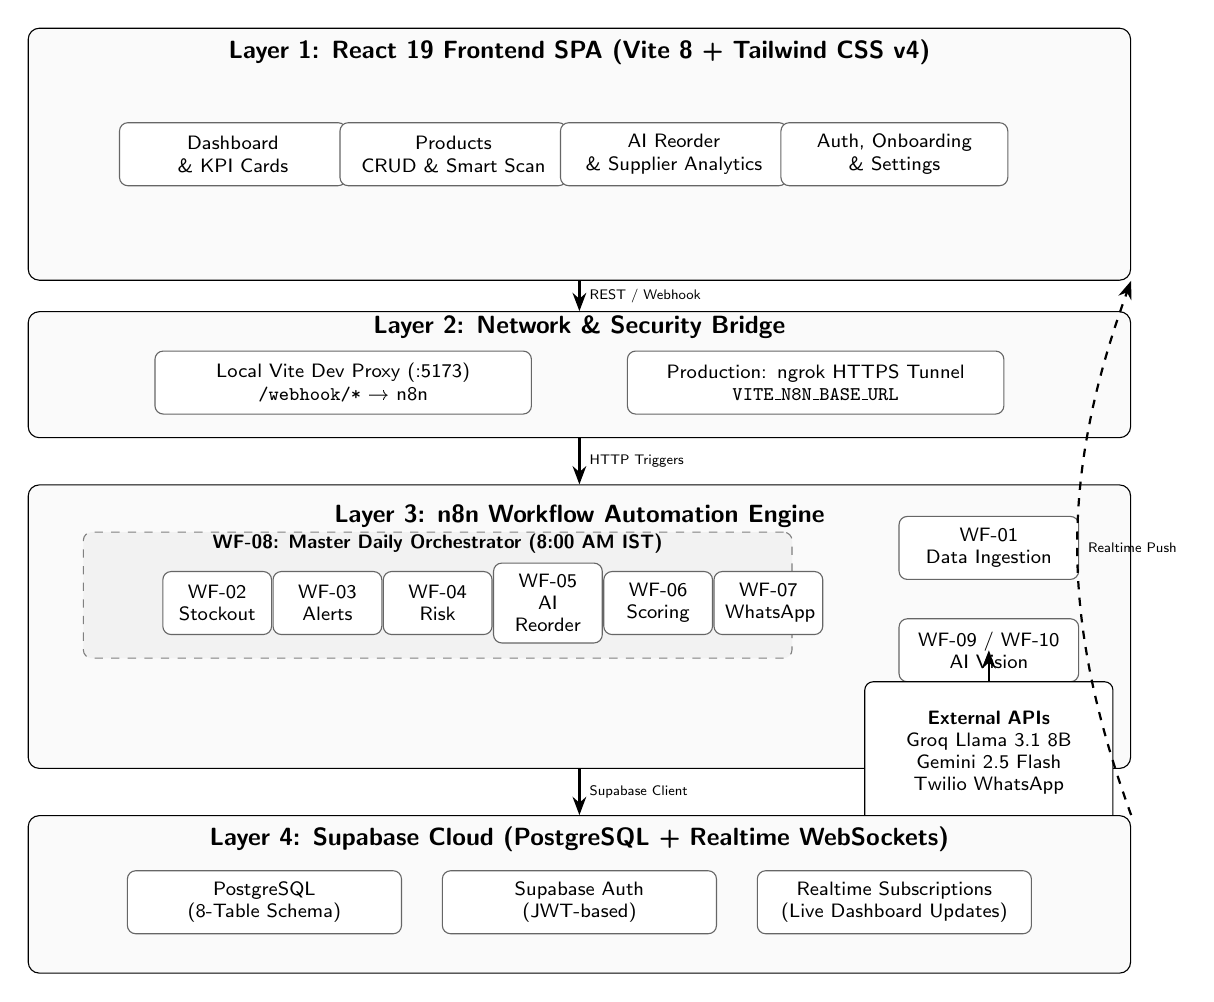
\begin{tikzpicture}[align=center,
  lyr/.style={rectangle, rounded corners=4pt, draw=black, fill=gray!4,
              minimum width=14cm, inner sep=8pt},
  box/.style={rectangle, rounded corners=3pt, draw=black!60, fill=white,
              font=\sffamily\scriptsize, inner sep=4pt, text width=2.6cm,
              minimum height=0.8cm, align=center},
  hdr/.style={font=\sffamily\small\bfseries},
  arr/.style={-Stealth, thick},
]

%% Layer 1 — Frontend
\node[lyr, minimum height=3.2cm] (L1) at (0,0) {};
\node[hdr] at (0, 1.3) {Layer 1: React 19 Frontend SPA (Vite 8 + Tailwind CSS v4)};
\node[box] at (-4.4, 0) {Dashboard\\\& KPI Cards};
\node[box] at (-1.6, 0) {Products\\CRUD \& Smart Scan};
\node[box] at (1.2, 0)  {AI Reorder\\\& Supplier Analytics};
\node[box] at (4.0, 0)  {Auth, Onboarding\\\& Settings};

%% Layer 2 — Network Bridge
\node[lyr, minimum height=1.6cm] (L2) at (0,-2.8) {};
\node[hdr] at (0, -2.2) {Layer 2: Network \& Security Bridge};
\node[box, text width=4.5cm] at (-3.0, -2.9) {Local Vite Dev Proxy (:5173)\\\texttt{/webhook/*} → n8n};
\node[box, text width=4.5cm] at (3.0, -2.9)  {Production: ngrok HTTPS Tunnel\\\texttt{VITE\_N8N\_BASE\_URL}};

%% Layer 3 — n8n Engine
\node[lyr, minimum height=3.6cm] (L3) at (0,-6.0) {};
\node[hdr] at (0, -4.6) {Layer 3: n8n Workflow Automation Engine};
% orchestrator sub-box
\node[rectangle, rounded corners=3pt, draw=black!50, fill=gray!10, dashed,
      minimum width=9.0cm, minimum height=1.6cm] at (-1.8, -5.6) {};
\node[font=\sffamily\scriptsize\bfseries] at (-1.8, -4.95) {WF-08: Master Daily Orchestrator (8:00 AM IST)};
\node[box, text width=1.1cm] at (-4.6,-5.7) {WF-02\\Stockout};
\node[box, text width=1.1cm] at (-3.2,-5.7) {WF-03\\Alerts};
\node[box, text width=1.1cm] at (-1.8,-5.7) {WF-04\\Risk};
\node[box, text width=1.1cm] at (-0.4,-5.7) {WF-05\\AI Reorder};
\node[box, text width=1.1cm] at (1.0,-5.7) {WF-06\\Scoring};
\node[box, text width=1.1cm] at (2.4,-5.7) {WF-07\\WhatsApp};
% standalone WFs
\node[box, text width=2.0cm] at (5.2, -5.0) {WF-01\\Data Ingestion};
\node[box, text width=2.0cm] at (5.2, -6.3) {WF-09 / WF-10\\AI Vision};

%% External APIs
\node[rectangle, rounded corners=3pt, draw=black, fill=white,
      font=\sffamily\scriptsize, inner sep=5pt, text width=2.8cm,
      align=center, minimum height=1.8cm] (API) at (5.2, -7.6)
  {\textbf{External APIs}\\Groq Llama 3.1 8B\\Gemini 2.5 Flash\\Twilio WhatsApp};

%% Layer 4 — Supabase
\node[lyr, minimum height=2.0cm] (L4) at (0,-9.4) {};
\node[hdr] at (0, -8.7) {Layer 4: Supabase Cloud (PostgreSQL + Realtime WebSockets)};
\node[box, text width=3.2cm] at (-4.0, -9.5) {PostgreSQL\\(8-Table Schema)};
\node[box, text width=3.2cm] at (0.0, -9.5)  {Supabase Auth\\(JWT-based)};
\node[box, text width=3.2cm] at (4.0, -9.5)  {Realtime Subscriptions\\(Live Dashboard Updates)};

%% Inter-layer arrows
\draw[arr] (L1.south) -- node[right,font=\sffamily\tiny]{REST / Webhook} (L2.north);
\draw[arr] (L2.south) -- node[right,font=\sffamily\tiny]{HTTP Triggers} (L3.north);
\draw[arr] (L3.south) -- node[right,font=\sffamily\tiny]{Supabase Client} (L4.north);
\draw[arr] (API.north) -- node[right,font=\sffamily\tiny]{} (5.2,-6.3);
\draw[arr,dashed] (L4.north east) to[bend left=20]
  node[right,font=\sffamily\tiny]{Realtime Push} (L1.south east);

\end{tikzpicture}%
}
\caption{Four-Layer System Architecture of StockSense AI.}
\label{fig:arch}
\end{figure}

The \textbf{Frontend Layer} is a React~19 single-page application bundled with Vite~8 and
styled using Tailwind CSS~v4. It presents twelve application routes covering the main dashboard,
product management, stock alert feed, AI reorder suggestions, supplier analytics, system logs,
and user settings. The frontend communicates with the n8n backend via REST webhooks and with
Supabase directly for authentication and real-time data subscriptions.

The \textbf{Network and Security Bridge Layer} handles the routing of frontend HTTP requests to
the appropriate backend destination. In the local development environment, a Vite reverse proxy
at port 5173 forwards all \texttt{/webhook/*} and \texttt{/api/v1/*} requests to the locally
hosted n8n instance, avoiding browser-imposed CORS restrictions. In production, an ngrok HTTPS
tunnel exposes the n8n instance to the internet, and the frontend environment variable
\texttt{VITE\_N8N\_BASE\_URL} is configured to point to the tunnel URL.

The \textbf{Workflow Engine Layer} comprises the ten n8n workflows that implement the core
business logic. WF-08, the Master Daily Orchestrator, executes at 8:00~AM IST and sequentially
calls WF-02 through WF-07 as sub-workflows. WF-01, WF-09, and WF-10 are webhook-triggered on
demand from the frontend.

The \textbf{Database Layer} is a Supabase PostgreSQL instance with an eight-table schema. Real-time
WebSocket subscriptions are enabled on the Products, Stock Alerts, Reorder Suggestions, Daily
Snapshots, Suppliers, and System Logs tables, ensuring that any change written by a workflow is
immediately reflected on the frontend without requiring a manual page refresh.

\section{Use Case Diagram Description}

The system recognises two principal actors: the \textbf{Store Owner} (primary user) and the
\textbf{n8n Automation Engine} (system actor). A third indirect actor, the \textbf{External AI
Services} (Groq, Gemini, Twilio), participates in sub-use cases triggered by the engine.

\begin{figure}[H]
\centering
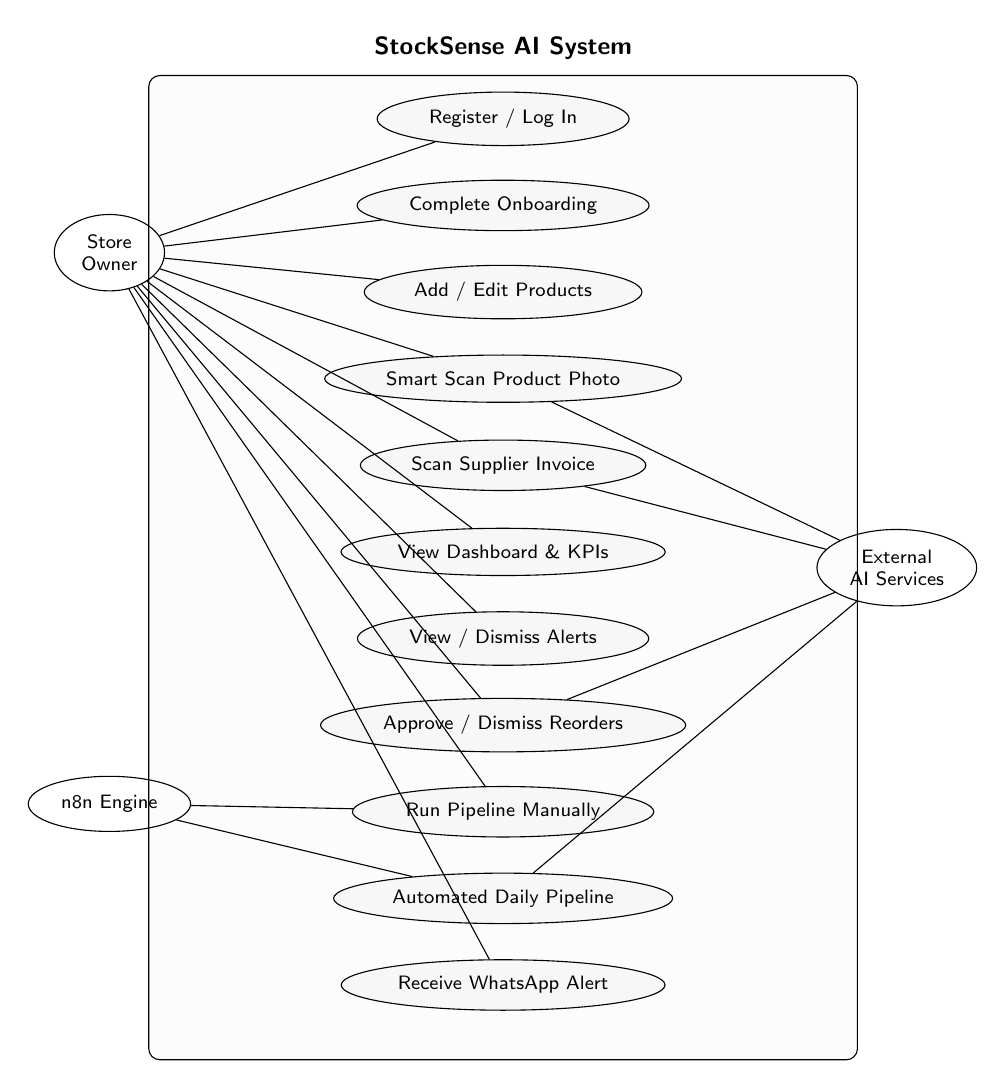
\begin{tikzpicture}[
  actor/.style={draw, ellipse, minimum width=1.4cm, minimum height=0.7cm,
                align=center, font=\sffamily\scriptsize},
  uc/.style={draw, ellipse, minimum width=3.2cm, minimum height=0.6cm,
             align=center, font=\sffamily\scriptsize, fill=gray!6},
  sys/.style={rectangle, rounded corners=4pt, draw=black, fill=gray!2,
              minimum width=9.0cm, minimum height=12.5cm},
  line/.style={draw, -}
]
% System boundary
\node[sys] at (3.5, 0) {};
\node[font=\sffamily\small\bfseries] at (3.5, 6.6) {StockSense AI System};

% Actors
\node[actor] (owner) at (-1.5, 4.0) {Store\\Owner};
\node[actor] (engine) at (-1.5, -3.0) {n8n Engine};
\node[actor] (ai) at (8.5, 0) {External\\AI Services};

% Use cases inside system
\node[uc] (uc1)  at (3.5,  5.7) {Register / Log In};
\node[uc] (uc2)  at (3.5,  4.6) {Complete Onboarding};
\node[uc] (uc3)  at (3.5,  3.5) {Add / Edit Products};
\node[uc] (uc4)  at (3.5,  2.4) {Smart Scan Product Photo};
\node[uc] (uc5)  at (3.5,  1.3) {Scan Supplier Invoice};
\node[uc] (uc6)  at (3.5,  0.2) {View Dashboard \& KPIs};
\node[uc] (uc7)  at (3.5, -0.9) {View / Dismiss Alerts};
\node[uc] (uc8)  at (3.5, -2.0) {Approve / Dismiss Reorders};
\node[uc] (uc9)  at (3.5, -3.1) {Run Pipeline Manually};
\node[uc] (uc10) at (3.5, -4.2) {Automated Daily Pipeline};
\node[uc] (uc11) at (3.5, -5.3) {Receive WhatsApp Alert};

% Connections — Store Owner
\foreach \t in {uc1,uc2,uc3,uc4,uc5,uc6,uc7,uc8,uc9,uc11}
  \draw[line] (owner) -- (\t);

% Connections — n8n Engine
\foreach \t in {uc10,uc9}
  \draw[line] (engine) -- (\t);

% Connections — AI Services
\foreach \t in {uc4,uc5,uc8,uc10}
  \draw[line] (ai) -- (\t);

\end{tikzpicture}
\caption{Use Case Diagram for StockSense AI.}
\label{fig:usecase}
\end{figure}

The Store Owner interacts with the system to manage products (add, edit, bulk import, smart scan),
review intelligence outputs (dashboard, alerts, reorder suggestions, supplier scores), and
configure the store profile and workflow settings. The n8n Engine initiates the daily orchestrated
pipeline and can be manually triggered by the Store Owner through the Settings page. External AI
Services are consumed by the engine during AI reorder generation (Groq), product and invoice
scanning (Gemini), and WhatsApp delivery (Twilio).

\section{Data Flow Diagram / ER Diagram}

\subsection{Data Flow Description}

The data flow through the StockSense AI pipeline proceeds as follows. When the Store Owner adds
or updates a product through the frontend, the form data is sent as a POST request to WF-01,
which validates the payload and performs an upsert operation on the Products table. When the
daily orchestrator (WF-08) fires at 8:00 AM IST, it first simulates the day's sales by
decrementing stock levels based on the \texttt{avg\_daily\_sales} value of each product. It
then sequentially invokes WF-02 to compute stockout dates, WF-03 to generate stock alerts for
products below threshold, WF-04 to classify risk levels, WF-05 to call Groq and write reorder
suggestions, WF-06 to recalculate supplier WSM scores, and WF-07 to dispatch WhatsApp messages
via Twilio. Upon completion, WF-08 calculates and saves the daily health snapshot and writes an
entry to System Logs. The Supabase Realtime WebSocket pushes all database changes to the
frontend instantly.

\subsection{Entity Relationship Description}

The central entity is the \textbf{Store Profile}, which acts as the multi-tenancy root and owns
all other entities through a \texttt{store\_id} foreign key. Each \textbf{Product} belongs to
one Store Profile, maintains its current stock level, average daily sales, risk classification,
and stockout projection. Each \textbf{Supplier} belongs to one Store Profile and carries
composite scoring information. \textbf{Stock Alerts} are generated per Product when
\texttt{current\_stock} $\leq$ \texttt{reorder\_threshold}. \textbf{Reorder Suggestions} link
a Product to a recommended Supplier and carry AI-generated reasoning. \textbf{Stock
Transactions} provide an immutable audit trail of all stock changes. \textbf{Daily Snapshots}
record aggregated health metrics per store per day. \textbf{System Logs} track the execution
status of each workflow run.

\begin{figure}[H]
\centering
\resizebox{\textwidth}{!}{%
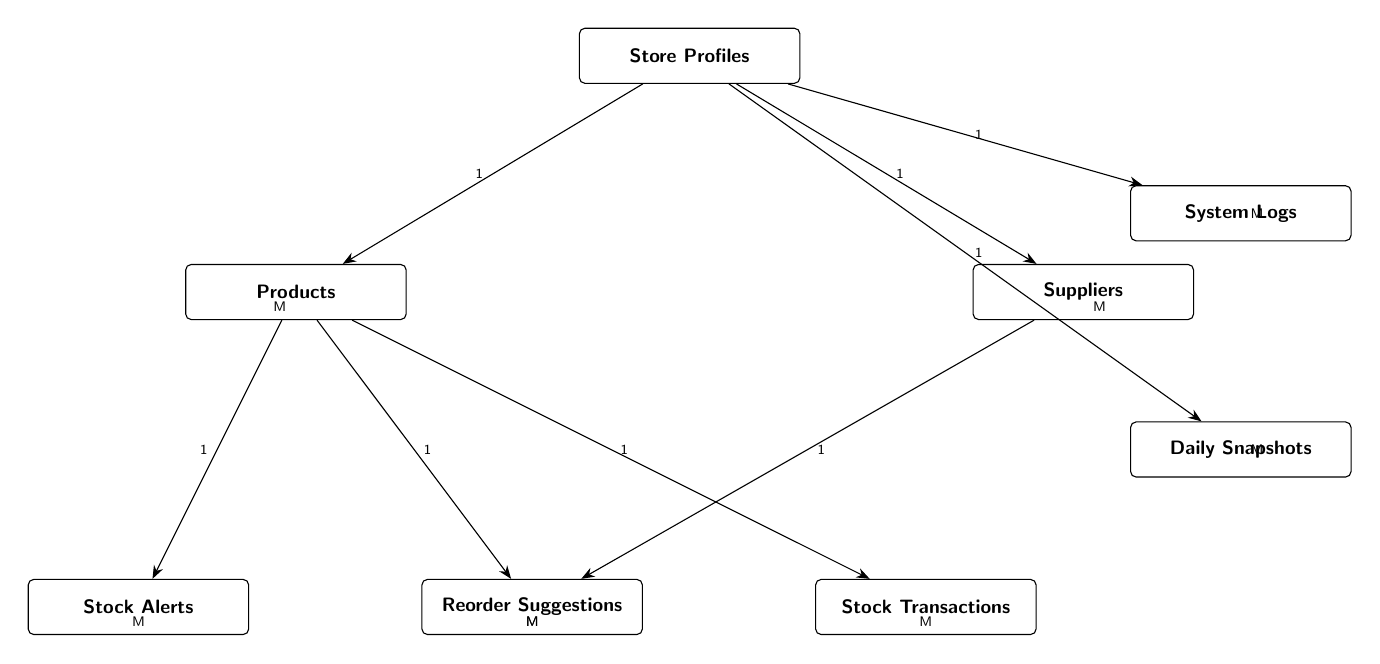
\begin{tikzpicture}[
  ent/.style={rectangle, draw=black, rounded corners=2pt, fill=white,
              font=\sffamily\scriptsize\bfseries, minimum width=2.8cm,
              minimum height=0.7cm, align=center},
  attr/.style={font=\sffamily\scriptsize, align=left},
  rel/.style={draw, -Stealth, font=\sffamily\tiny},
]
% Entities
\node[ent] (SP) at (0,0) {Store Profiles};
\node[ent] (PR) at (-5,-3) {Products};
\node[ent] (SU) at (5,-3) {Suppliers};
\node[ent] (SA) at (-7,-7) {Stock Alerts};
\node[ent] (RS) at (-2,-7) {Reorder Suggestions};
\node[ent] (ST) at (3,-7) {Stock Transactions};
\node[ent] (DS) at (7,-5) {Daily Snapshots};
\node[ent] (SL) at (7,-2) {System Logs};

% Relationships
\draw[rel] (SP) -- node[left,font=\sffamily\tiny]{1} (PR) node[below left,font=\sffamily\tiny]{M};
\draw[rel] (SP) -- node[right,font=\sffamily\tiny]{1} (SU) node[below right,font=\sffamily\tiny]{M};
\draw[rel] (SP) -- node[right,font=\sffamily\tiny]{1} (SL) node[right,font=\sffamily\tiny]{M};
\draw[rel] (SP) -- node[right,font=\sffamily\tiny]{1} (DS) node[right,font=\sffamily\tiny]{M};
\draw[rel] (PR) -- node[left,font=\sffamily\tiny]{1} (SA) node[below,font=\sffamily\tiny]{M};
\draw[rel] (PR) -- node[right,font=\sffamily\tiny]{1} (RS) node[below,font=\sffamily\tiny]{M};
\draw[rel] (PR) -- node[right,font=\sffamily\tiny]{1} (ST) node[below,font=\sffamily\tiny]{M};
\draw[rel] (SU) -- node[right,font=\sffamily\tiny]{1} (RS) node[below,font=\sffamily\tiny]{M};
\end{tikzpicture}%
}
\caption{Entity Relationship Diagram for StockSense AI Database.}
\label{fig:erd}
\end{figure}

\section{Module Description}

StockSense AI is decomposed into six functional modules, each encapsulating a coherent set of
responsibilities:

\textbf{Module 1 — Data Ingestion and Product Management:} Handles all CRUD operations on the
Products table. Includes the frontend Add/Edit Product modal, CSV bulk import functionality,
AI Smart Scan (WF-09), and the Quick Update batch stock adjustment page. The underlying WF-01
webhook processes all inbound product data.

\textbf{Module 2 — Inventory Intelligence Pipeline:} The core analytical engine comprising
WF-02 (Stockout Prediction), WF-03 (Alert Generation), WF-04 (Risk Classification), and
WF-08 (Daily Orchestrator). This module runs autonomously on a schedule and updates the database
with fresh intelligence data for every product.

\textbf{Module 3 — AI Reorder Recommendations:} WF-05 implements the Groq API integration.
It constructs a structured zero-shot prompt from current inventory and supplier data and parses
the JSON array response into Reorder Suggestion records. The frontend Reorder page displays these
suggestions and allows the Store Owner to approve or dismiss them.

\textbf{Module 4 — Supplier Scoring and Analytics:} WF-06 computes the Weighted Sum Model score
for each supplier and assigns letter grades. The Suppliers page visualises composite scores,
individual metric breakdowns, and grade badges.

\textbf{Module 5 — WhatsApp Alert Delivery:} WF-07 queries active Stock Alerts, applies a
24-hour anti-spam filter based on \texttt{last\_alerted\_at} timestamps, formats a message
containing the critical product list, and delivers it via Twilio's WhatsApp Business API.

\textbf{Module 6 — AI Vision Data Entry:} WF-09 accepts base64-encoded product photographs,
uses Gemini~2.5 Flash to extract product name and category, and returns auto-populated form
data to the frontend. WF-10 processes supplier invoice photographs, extracting product names
and quantities, and uses fuzzy string matching to map them to existing inventory records.

\section{Database Design}

The complete database schema consists of eight tables hosted on Supabase PostgreSQL. All primary
keys use UUID values generated by \texttt{gen\_random\_uuid()}. All tables include a
\texttt{created\_at} timestamp. All data-bearing tables include a \texttt{store\_id} foreign
key referencing Store Profiles, enabling multi-tenant extension.

\begin{table}[H]
\centering
\caption{Database Table Summary}
\label{tab:dbsummary}
{\singlespacing
\begin{tabularx}{\textwidth}{@{} l X l @{}}
\toprule
\textbf{Table} & \textbf{Purpose} & \textbf{Key Columns} \\
\midrule
Store Profiles  & Multi-tenancy root; one record per registered store &
  \texttt{user\_id}, \texttt{store\_name}, \texttt{whatsapp\_numbers}, \texttt{safety\_factor} \\
\addlinespace
Products        & Inventory item master with live intelligence fields &
  \texttt{product\_id}, \texttt{current\_stock}, \texttt{avg\_daily\_sales},
  \texttt{days\_to\_stockout}, \texttt{risk\_level} \\
\addlinespace
Suppliers       & Vendor directory with scoring outputs &
  \texttt{supplier\_id}, \texttt{reliability\_score}, \texttt{price\_score},
  \texttt{composite\_score}, \texttt{supplier\_grade} \\
\addlinespace
Stock Alerts    & Active low-stock alerts (stock $\leq$ threshold) &
  \texttt{product\_id}, \texttt{alert\_status}, \texttt{last\_alerted\_at} \\
\addlinespace
Reorder Suggestions & AI-generated reorder recommendations &
  \texttt{product\_id}, \texttt{supplier\_id}, \texttt{suggested\_quantity}, \texttt{reason},
  \texttt{status} \\
\addlinespace
Stock Transactions & Immutable audit log of all stock changes &
  \texttt{transaction\_type}, \texttt{quantity\_change}, \texttt{new\_stock\_level} \\
\addlinespace
Daily Snapshots & Historical daily health metrics per store &
  \texttt{snapshot\_date}, \texttt{health\_score}, \texttt{high\_count}, \texttt{oos\_count} \\
\addlinespace
System Logs     & Workflow execution records &
  \texttt{workflow\_name}, \texttt{status}, \texttt{records\_processed}, \texttt{error\_message} \\
\bottomrule
\end{tabularx}
}
\end{table}

Real-time Supabase subscriptions are enabled on Products, Stock Alerts, Reorder Suggestions,
Daily Snapshots, Suppliers, and System Logs. Indexed columns include \texttt{product\_id},
\texttt{risk\_level}, \texttt{alert\_status}, and \texttt{snapshot\_date} for query performance.
Row-level security policies are not enforced in the prototype but the schema is designed to
support them for production multi-tenancy deployment.

% =============================================================================
% CHAPTER 4 — IMPLEMENTATION
% =============================================================================
\chapter{Implementation}
\label{ch:impl}

\section{Technology Stack and Justification}

The technology choices for StockSense AI were governed by three criteria: cost, accessibility,
and capability. Each component of the stack was selected because it satisfies all three criteria
simultaneously. Table~\ref{tab:stack} presents the complete technology stack.

{\singlespacing
\renewcommand{\arraystretch}{1.5}
\begin{longtable}{@{} >{\raggedright\arraybackslash}p{3.5cm} >{\raggedright\arraybackslash}p{2.5cm} >{\raggedright\arraybackslash}p{8.5cm} @{}}
\caption{Technology Stack and Justification}
\label{tab:stack} \\
\toprule
\textbf{Technology} & \textbf{Role} & \textbf{Justification} \\
\midrule
\endfirsthead
\toprule
\textbf{Technology} & \textbf{Role} & \textbf{Justification} \\
\midrule
\endhead
\bottomrule
\endfoot
React 19 & Frontend framework &
  Component-based architecture; Concurrent Mode rendering for real-time UI updates;
  large ecosystem and strong community support. \\
Vite 8 & Build tool &
  Sub-second hot module replacement; built-in reverse proxy eliminates CORS issues
  in development; fast production bundle generation. \\
Tailwind CSS v4 & Styling &
  Utility-first CSS with the new \texttt{@theme} directive eliminates need for a
  separate configuration file; consistent design tokens across all components. \\
React Router 7 & Client routing &
  Declarative route definitions; nested layouts with \texttt{Outlet}; programmatic
  navigation for post-auth redirection. \\
Supabase & Database + Auth &
  Managed PostgreSQL with built-in authentication, real-time WebSocket subscriptions,
  and a JavaScript client; generous free tier; no server management required. \\
n8n (self-hosted) & Workflow engine &
  Low-code automation with visual workflow editor; native HTTP, Supabase, Groq,
  and Twilio integrations; cron scheduler for daily orchestration. \\
Groq Llama 3.1 8B & LLM inference &
  Fastest available inference speed for the Llama~3.1 family; free tier with
  generous rate limits suitable for prototype; JSON output mode for reliable parsing. \\
Google Gemini 2.5 Flash & Multimodal AI &
  State-of-the-art vision-language model for image understanding; supports base64
  image input; reliable JSON structured output for product and invoice extraction. \\
Twilio WhatsApp API & Alert delivery &
  Industry-standard CPaaS with sandbox WhatsApp support; simple REST API; per-message
  pricing model viable at kirana store scale. \\
ngrok & Tunnelling &
  HTTPS tunnel for exposing local n8n instance; used in development and
  early production; replaced by cloud hosting for persistent deployment. \\
\end{longtable}
}

\section{Development Environment}

The development environment was configured as follows:

\begin{itemize}[itemsep=3pt]
  \item \textbf{Operating System:} Windows 11 with PowerShell 7
  \item \textbf{Node.js:} v22 LTS (required for Vite 8 and React 19)
  \item \textbf{Package Manager:} npm with \texttt{--legacy-peer-deps} flag due to
        React 19 peer dependency resolution requirements
  \item \textbf{n8n:} Self-hosted via \texttt{npx n8n} on \texttt{localhost:5678}
  \item \textbf{Supabase:} Cloud-hosted project (free tier) accessed via the JavaScript
        client library \texttt{@supabase/supabase-js}
  \item \textbf{Environment Variables:} Stored in \texttt{frontend/.env} with
        \texttt{VITE\_} prefix for Vite client-side injection:
        \texttt{VITE\_SUPABASE\_URL}, \texttt{VITE\_SUPABASE\_ANON\_KEY},
        \texttt{VITE\_N8N\_BASE\_URL}, \texttt{VITE\_N8N\_API\_KEY}
  \item \textbf{Code Editor:} Visual Studio Code with ESLint extension
  \item \textbf{ESLint:} Flat config (ESLint 9) with
        \texttt{eslint-plugin-react-hooks} and \texttt{eslint-plugin-react-refresh}
  \item \textbf{Version Control:} Git with GitHub remote; single \texttt{main} branch;
        Conventional Commits message format
\end{itemize}

The Vite development server is configured to proxy all requests matching \texttt{/webhook/*}
and \texttt{/api/v1/*} to the n8n instance URL defined in \texttt{VITE\_N8N\_BASE\_URL},
eliminating browser-imposed CORS rejections without requiring changes to n8n's own CORS
configuration.

\section{Module-wise Implementation}

\subsection{WF-01: Product and Sales Data Ingestion}

WF-01 exposes a POST webhook at \texttt{/webhook/product-sales-ingest}. Upon receiving a
request from the frontend Add Product form, the workflow cleans and normalises the incoming
fields (removing whitespace, setting default values for optional fields), performs a lookup of
the Products table by \texttt{product\_id}, and branches on existence. If the product already
exists, it executes an UPDATE operation; if not, it inserts a new row. The webhook then responds
with a success payload that the frontend uses to dismiss the modal and trigger a real-time
refresh.

\begin{figure}[H]
\centering
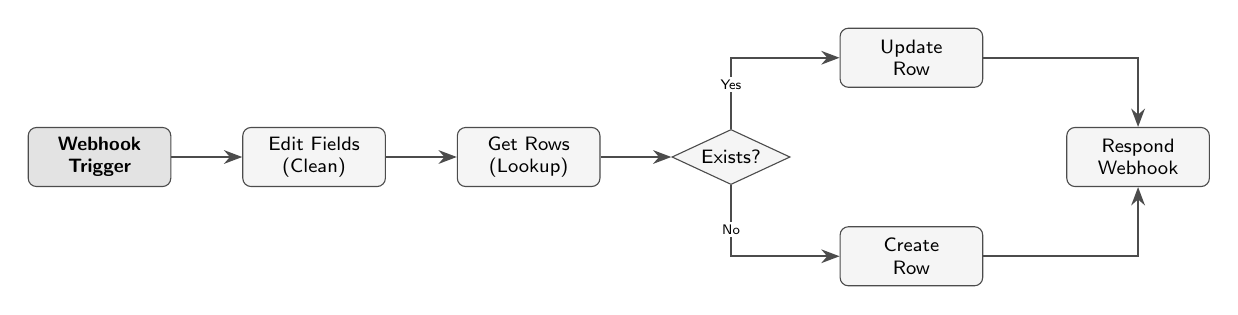
\begin{tikzpicture}[node distance=0.5cm and 0.9cm, align=center]
  \node (n1) [wftrigger] {Webhook\\Trigger};
  \node (n2) [wfnode, right=of n1] {Edit Fields\\(Clean)};
  \node (n3) [wfnode, right=of n2] {Get Rows\\(Lookup)};
  \node (n4) [wfdecision, right=of n3] {Exists?};
  \node (n5a) [wfnode, above right=0.7cm and 1.0cm of n4] {Update\\Row};
  \node (n5b) [wfnode, below right=0.7cm and 1.0cm of n4] {Create\\Row};
  \node (n6) [wfnode, right=3.5cm of n4] {Respond\\Webhook};
  \draw[wfarrow] (n1)--(n2); \draw[wfarrow] (n2)--(n3); \draw[wfarrow] (n3)--(n4);
  \draw[wfarrow] (n4) |- node[wflabel,pos=0.25,above]{Yes} (n5a);
  \draw[wfarrow] (n4) |- node[wflabel,pos=0.25,below]{No}  (n5b);
  \draw[wfarrow] (n5a) -| (n6); \draw[wfarrow] (n5b) -| (n6);
\end{tikzpicture}
\caption{WF-01: Product and Sales Data Ingestion Workflow.}
\label{fig:wf01}
\end{figure}

\subsection{WF-02: Stockout Date Calculator}

WF-02 fetches all products from the Products table and applies the stockout prediction
formula. For each product, the workflow computes:

\begin{equation}
d_{\text{stockout}} = \left\lfloor \frac{S_{\text{current}}}{V_{\text{daily}}} \right\rfloor, \quad
\text{date}_{\text{stockout}} = \text{date}_{\text{today}} + d_{\text{stockout}}
\label{eq:stockout}
\end{equation}

Edge cases are handled explicitly: if $V_{\text{daily}} = 0$, then $d_{\text{stockout}}$ is set
to 999 (interpreted as "no foreseeable stockout"); if $S_{\text{current}} = 0$, then
$d_{\text{stockout}} = 0$ (immediate stockout). Both \texttt{days\_to\_stockout} and
\texttt{estimated\_stockout\_date} are written back to each product row.

\begin{figure}[H]
\centering
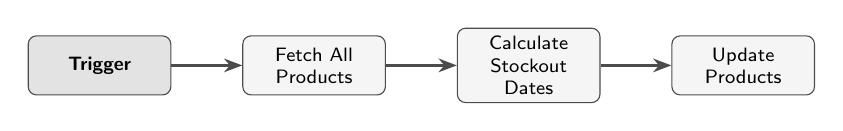
\begin{tikzpicture}[node distance=0.5cm and 0.9cm, align=center]
  \node (n1) [wftrigger] {Trigger};
  \node (n2) [wfnode, right=of n1] {Fetch All\\Products};
  \node (n3) [wfnode, right=of n2] {Calculate\\Stockout Dates};
  \node (n4) [wfnode, right=of n3] {Update\\Products};
  \draw[wfarrow] (n1)--(n2); \draw[wfarrow] (n2)--(n3); \draw[wfarrow] (n3)--(n4);
\end{tikzpicture}
\caption{WF-02: Stockout Date Calculator Workflow.}
\label{fig:wf02}
\end{figure}

\subsection{WF-03: Inventory Processing and Stock Alerts}

WF-03 identifies all products where \texttt{current\_stock} $\leq$ \texttt{reorder\_threshold}.
It first deletes all existing Stock Alert rows for the store (a clean-slate refresh strategy),
then inserts fresh alert records for each at-risk product with status \texttt{ACTIVE}. This
approach avoids duplicate alert accumulation and ensures the alert feed always reflects the
current inventory state.

\begin{figure}[H]
\centering
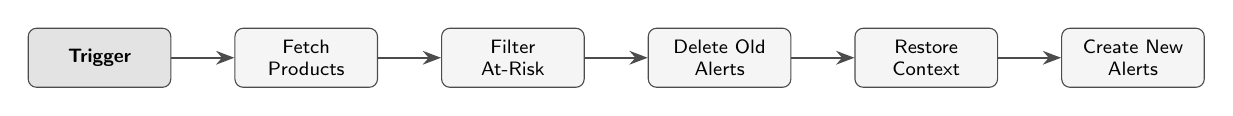
\begin{tikzpicture}[node distance=0.5cm and 0.8cm, align=center]
  \node (n1) [wftrigger] {Trigger};
  \node (n2) [wfnode, right=of n1] {Fetch\\Products};
  \node (n3) [wfnode, right=of n2] {Filter\\At-Risk};
  \node (n4) [wfnode, right=of n3] {Delete Old\\Alerts};
  \node (n5) [wfnode, right=of n4] {Restore\\Context};
  \node (n6) [wfnode, right=of n5] {Create New\\Alerts};
  \draw[wfarrow] (n1)--(n2); \draw[wfarrow] (n2)--(n3);
  \draw[wfarrow] (n3)--(n4); \draw[wfarrow] (n4)--(n5); \draw[wfarrow] (n5)--(n6);
\end{tikzpicture}
\caption{WF-03: Inventory Processing and Stock Alert Generation Workflow.}
\label{fig:wf03}
\end{figure}

\subsection{WF-04: Stock Risk Classification}

WF-04 classifies each product into one of four risk tiers using the following piecewise function
applied to \texttt{days\_to\_stockout}:

\begin{equation}
\text{risk} =
\begin{cases}
\text{HIGH}    & \text{if } d_{\text{stockout}} \leq 3 \\
\text{MEDIUM}  & \text{if } 3 < d_{\text{stockout}} \leq 7 \\
\text{LOW}     & \text{if } d_{\text{stockout}} > 7 \\
\text{UNKNOWN} & \text{if stockout data unavailable}
\end{cases}
\label{eq:risk}
\end{equation}

The classified risk level is written back to the \texttt{risk\_level} column of each product row
and is used by the frontend dashboard to colour-code product cards and by WF-05 to filter
at-risk products for AI reorder suggestion generation.

\begin{figure}[H]
\centering
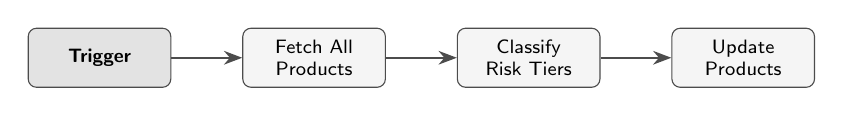
\begin{tikzpicture}[node distance=0.5cm and 0.9cm, align=center]
  \node (n1) [wftrigger] {Trigger};
  \node (n2) [wfnode, right=of n1] {Fetch All\\Products};
  \node (n3) [wfnode, right=of n2] {Classify\\Risk Tiers};
  \node (n4) [wfnode, right=of n3] {Update\\Products};
  \draw[wfarrow] (n1)--(n2); \draw[wfarrow] (n2)--(n3); \draw[wfarrow] (n3)--(n4);
\end{tikzpicture}
\caption{WF-04: Stock Risk Classification Workflow.}
\label{fig:wf04}
\end{figure}

\subsection{WF-05: AI Reorder Intelligence}

WF-05 constitutes the most sophisticated workflow in the pipeline. It fetches at-risk products
(risk level HIGH or MEDIUM) and all suppliers in parallel, merges the two data streams, and
constructs a structured zero-shot prompt for the Groq Llama~3.1~8B model. The prompt
instructs the model to act as an inventory manager for an Indian kirana store and to return
a JSON array of reorder suggestions, one per at-risk product, with fields:
\texttt{product\_id}, \texttt{supplier\_id}, \texttt{suggested\_qty}
($= 30 \times V_{\text{daily}}$), and \texttt{reason} (one-sentence justification).

\begin{figure}[H]
\centering
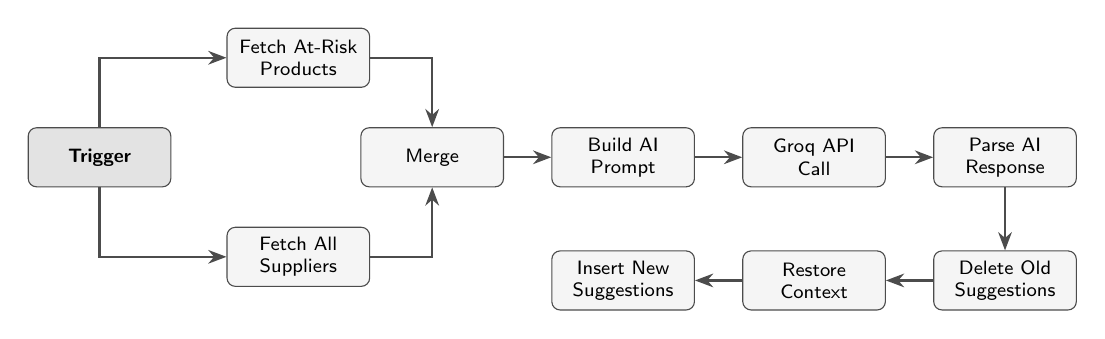
\begin{tikzpicture}[node distance=0.5cm and 0.6cm, align=center]
  \node (n1) [wftrigger] {Trigger};
  \node (n2a) [wfnode, above right=0.5cm and 0.7cm of n1] {Fetch At-Risk\\Products};
  \node (n2b) [wfnode, below right=0.5cm and 0.7cm of n1] {Fetch All\\Suppliers};
  \node (n3) [wfnode, right=2.4cm of n1] {Merge};
  \node (n4) [wfnode, right=of n3] {Build AI\\Prompt};
  \node (n5) [wfnode, right=of n4] {Groq API\\Call};
  \node (n6) [wfnode, right=of n5] {Parse AI\\Response};
  \node (n7) [wfnode, below=0.8cm of n6] {Delete Old\\Suggestions};
  \node (n8) [wfnode, left=of n7] {Restore\\Context};
  \node (n9) [wfnode, left=of n8] {Insert New\\Suggestions};
  \draw[wfarrow] (n1) |- (n2a); \draw[wfarrow] (n1) |- (n2b);
  \draw[wfarrow] (n2a) -| (n3); \draw[wfarrow] (n2b) -| (n3);
  \draw[wfarrow] (n3)--(n4); \draw[wfarrow] (n4)--(n5);
  \draw[wfarrow] (n5)--(n6); \draw[wfarrow] (n6)--(n7);
  \draw[wfarrow] (n7)--(n8); \draw[wfarrow] (n8)--(n9);
\end{tikzpicture}
\caption{WF-05: AI Reorder Intelligence Workflow.}
\label{fig:wf05}
\end{figure}

\subsection{WF-06: Supplier Scoring}

WF-06 evaluates all suppliers using the Weighted Sum Model. The composite score $C_s$ is
computed as:

\begin{equation}
C_s = (R \times 0.40 + P \times 0.35 + D \times 0.25) \times 100
\label{eq:wsm}
\end{equation}

where $R$ is the reliability score (0--1), $P$ is the price score (0--1), and $D$ is the
delivery speed score (min-max normalised: fastest supplier $= 1.0$, slowest $= 0.0$). Letter
grades are assigned as: A ($C_s \geq 80$), B ($65 \leq C_s < 80$), C ($50 \leq C_s < 65$),
D ($C_s < 50$). Both score and grade are written to the Suppliers table.

\begin{figure}[H]
\centering
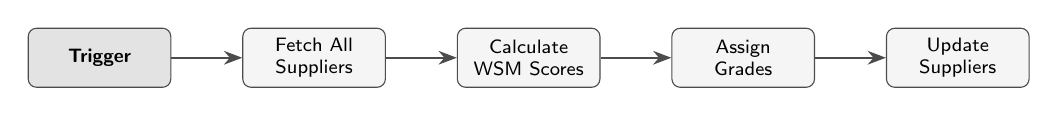
\begin{tikzpicture}[node distance=0.5cm and 0.9cm, align=center]
  \node (n1) [wftrigger] {Trigger};
  \node (n2) [wfnode, right=of n1] {Fetch All\\Suppliers};
  \node (n3) [wfnode, right=of n2] {Calculate\\WSM Scores};
  \node (n4) [wfnode, right=of n3] {Assign\\Grades};
  \node (n5) [wfnode, right=of n4] {Update\\Suppliers};
  \draw[wfarrow] (n1)--(n2); \draw[wfarrow] (n2)--(n3);
  \draw[wfarrow] (n3)--(n4); \draw[wfarrow] (n4)--(n5);
\end{tikzpicture}
\caption{WF-06: Supplier Scoring Workflow.}
\label{fig:wf06}
\end{figure}

\subsection{WF-07: WhatsApp Alert Sender}

WF-07 queries the Stock Alerts table for all records with \texttt{alert\_status = 'ACTIVE'}.
It applies a 24-hour anti-spam filter by checking \texttt{last\_alerted\_at}: only products
not alerted in the last 24 hours proceed to the message builder. A formatted WhatsApp message
is constructed listing all qualifying products with their names, current stock, and threshold
values. The message is dispatched to the registered store WhatsApp numbers via the Twilio
Messages API. After successful delivery, \texttt{last\_alerted\_at} is updated for each
product.

\begin{figure}[H]
\centering
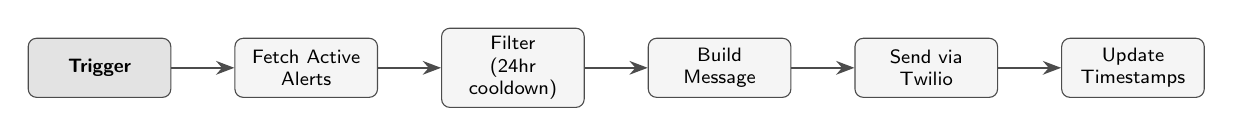
\begin{tikzpicture}[node distance=0.5cm and 0.8cm, align=center]
  \node (n1) [wftrigger] {Trigger};
  \node (n2) [wfnode, right=of n1] {Fetch Active\\Alerts};
  \node (n3) [wfnode, right=of n2] {Filter\\(24hr cooldown)};
  \node (n4) [wfnode, right=of n3] {Build\\Message};
  \node (n5) [wfnode, right=of n4] {Send via\\Twilio};
  \node (n6) [wfnode, right=of n5] {Update\\Timestamps};
  \draw[wfarrow] (n1)--(n2); \draw[wfarrow] (n2)--(n3); \draw[wfarrow] (n3)--(n4);
  \draw[wfarrow] (n4)--(n5); \draw[wfarrow] (n5)--(n6);
\end{tikzpicture}
\caption{WF-07: WhatsApp Alert Sender Workflow.}
\label{fig:wf07}
\end{figure}

\subsection{WF-08: Master Daily Orchestrator}

WF-08 is triggered by an n8n Cron node set to 8:00 AM IST daily. It begins by simulating the
day's sales by subtracting each product's \texttt{avg\_daily\_sales} from its
\texttt{current\_stock} (with a floor of zero). It then sequentially executes WF-02 through
WF-07 as sub-workflow calls, waiting for each to complete before proceeding. After WF-07
completes, WF-08 computes the daily health score using the inventory health formula and inserts
a Daily Snapshot record. Finally, it writes a completion entry to System Logs.

\begin{figure}[H]
\centering
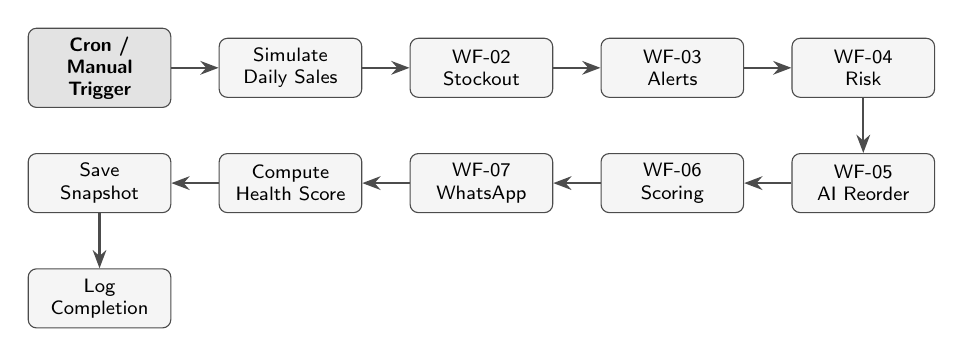
\begin{tikzpicture}[node distance=0.45cm and 0.6cm, align=center]
  \node (t)   [wftrigger] {Cron / Manual\\Trigger};
  \node (sim) [wfnode, right=of t]  {Simulate\\Daily Sales};
  \node (w2)  [wfnode, right=of sim] {WF-02\\Stockout};
  \node (w3)  [wfnode, right=of w2]  {WF-03\\Alerts};
  \node (w4)  [wfnode, right=of w3]  {WF-04\\Risk};
  \node (w5)  [wfnode, below=0.7cm of w4] {WF-05\\AI Reorder};
  \node (w6)  [wfnode, left=of w5]  {WF-06\\Scoring};
  \node (w7)  [wfnode, left=of w6]  {WF-07\\WhatsApp};
  \node (hs)  [wfnode, left=of w7]  {Compute\\Health Score};
  \node (sn)  [wfnode, left=of hs]  {Save\\Snapshot};
  \node (lg)  [wfnode, below=0.7cm of sn] {Log\\Completion};
  \draw[wfarrow] (t)--(sim); \draw[wfarrow] (sim)--(w2); \draw[wfarrow] (w2)--(w3);
  \draw[wfarrow] (w3)--(w4); \draw[wfarrow] (w4)--(w5); \draw[wfarrow] (w5)--(w6);
  \draw[wfarrow] (w6)--(w7); \draw[wfarrow] (w7)--(hs); \draw[wfarrow] (hs)--(sn);
  \draw[wfarrow] (sn)--(lg);
\end{tikzpicture}
\caption{WF-08: Master Daily Orchestrator Workflow.}
\label{fig:wf08}
\end{figure}

\subsection{WF-09: AI Vision Product Onboarding}

WF-09 exposes a POST webhook that accepts a base64-encoded image of a product. The image is
passed directly to the Gemini~2.5 Flash multimodal API with a structured prompt requesting
extraction of \texttt{product\_name} and \texttt{category} in JSON format. A recursive parser
handles Gemini's response envelope to reliably extract the JSON payload regardless of any
markdown fencing or preamble. The workflow then queries the Products table to determine the
highest existing product ID suffix and returns an auto-incremented collision-free ID along
with the extracted fields to the frontend form.

\begin{figure}[H]
\centering
\resizebox{\textwidth}{!}{%
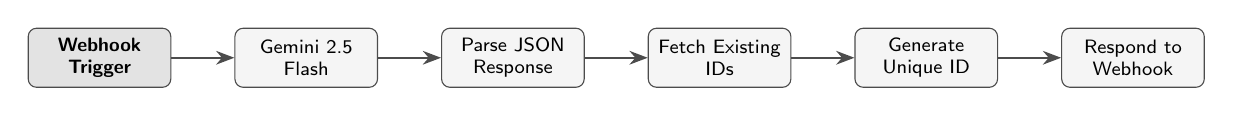
\begin{tikzpicture}[node distance=0.5cm and 0.8cm, align=center]
  \node (n1) [wftrigger] {Webhook\\Trigger};
  \node (n2) [wfnode, right=of n1] {Gemini 2.5\\Flash};
  \node (n3) [wfnode, right=of n2] {Parse JSON\\Response};
  \node (n4) [wfnode, right=of n3] {Fetch Existing\\IDs};
  \node (n5) [wfnode, right=of n4] {Generate\\Unique ID};
  \node (n6) [wfnode, right=of n5] {Respond to\\Webhook};
  \draw[wfarrow] (n1)--(n2); \draw[wfarrow] (n2)--(n3); \draw[wfarrow] (n3)--(n4);
  \draw[wfarrow] (n4)--(n5); \draw[wfarrow] (n5)--(n6);
\end{tikzpicture}%
}
\caption{WF-09: AI Vision Onboarding Workflow.}
\label{fig:wf09}
\end{figure}

\subsection{WF-10: Smart Scan for Supplier Invoices}

WF-10 processes photographs of physical supplier delivery bills. The image is submitted to
Gemini~2.5 Flash with a prompt requesting extraction of all line items as a JSON array of
\texttt{\{product\_name, quantity\}} objects. The extracted items are then matched against
the store's existing Products table using a fuzzy string similarity algorithm implemented in
an n8n Code node. The algorithm computes character-level similarity scores between each
extracted product name and all inventory product names, selecting the best match above a
defined confidence threshold. The matched product IDs and computed new stock levels are
returned to the frontend for the store owner to review and confirm.

\begin{figure}[H]
\centering
\resizebox{\textwidth}{!}{%
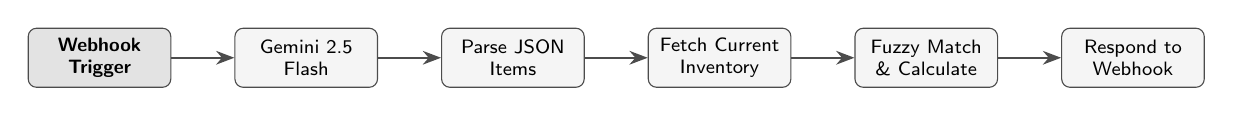
\begin{tikzpicture}[node distance=0.5cm and 0.8cm, align=center]
  \node (n1) [wftrigger] {Webhook\\Trigger};
  \node (n2) [wfnode, right=of n1] {Gemini 2.5\\Flash};
  \node (n3) [wfnode, right=of n2] {Parse JSON\\Items};
  \node (n4) [wfnode, right=of n3] {Fetch Current\\Inventory};
  \node (n5) [wfnode, right=of n4] {Fuzzy Match\\\& Calculate};
  \node (n6) [wfnode, right=of n5] {Respond to\\Webhook};
  \draw[wfarrow] (n1)--(n2); \draw[wfarrow] (n2)--(n3); \draw[wfarrow] (n3)--(n4);
  \draw[wfarrow] (n4)--(n5); \draw[wfarrow] (n5)--(n6);
\end{tikzpicture}%
}
\caption{WF-10: Smart Scan Invoice Workflow.}
\label{fig:wf10}
\end{figure}

\section{Key Code Snippets with Explanation}

\subsection{Stockout Calculation Logic (n8n Code Node)}

The following JavaScript implements the stockout prediction formula within the WF-02 Code node:

\begin{lstlisting}[language=javascript, caption={WF-02 Stockout Calculation Code Node}, label={lst:stockout}]
const items = $input.all();
const today = new Date().toISOString().split('T')[0];

return items.map(item => {
  const { current_stock, avg_daily_sales } = item.json;
  const stock  = parseFloat(current_stock)  || 0;
  const sales  = parseFloat(avg_daily_sales) || 0;

  let days;
  if (stock === 0)    { days = 0; }
  else if (sales === 0) { days = 999; }
  else                { days = Math.floor(stock / sales); }

  const stockoutDate = new Date();
  stockoutDate.setDate(stockoutDate.getDate() + days);

  return {
    json: {
      ...item.json,
      days_to_stockout: days,
      estimated_stockout_date:
        days === 999 ? null : stockoutDate.toISOString().split('T')[0],
    }
  };
});
\end{lstlisting}

The \texttt{Math.floor} operation matches Equation~\ref{eq:stockout} precisely. The ternary
guard for \texttt{avg\_daily\_sales = 0} prevents division-by-zero errors in production.

\subsection{Supplier WSM Scoring Logic (n8n Code Node)}

\begin{lstlisting}[language=javascript, caption={WF-06 Weighted Sum Model Scoring}, label={lst:wsm}]
const suppliers = $input.all().map(i => i.json);

// Min-max normalise delivery time (faster = higher score)
const times = suppliers.map(s => s.delivery_time_days);
const minT  = Math.min(...times);
const maxT  = Math.max(...times);

return suppliers.map(s => {
  const R = parseFloat(s.reliability_score);
  const P = parseFloat(s.price_score);
  const D = maxT === minT ? 1 :
    (maxT - s.delivery_time_days) / (maxT - minT);

  const score = (R * 0.40 + P * 0.35 + D * 0.25) * 100;
  const grade = score >= 80 ? 'A' : score >= 65 ? 'B' :
                score >= 50 ? 'C' : 'D';

  return { json: { ...s, composite_score: score.toFixed(2),
                         supplier_grade: grade } };
});
\end{lstlisting}

\subsection{Supabase Realtime Subscription Pattern (React)}

All pages that display live data use the following pattern to subscribe to database changes:

\begin{lstlisting}[language=javascript, caption={Supabase Realtime Subscription Pattern}, label={lst:realtime}]
useEffect(() => {
  fetchProducts();          // initial data load
  const channel = supabase
    .channel('products-live')
    .on('postgres_changes',
        { event: '*', schema: 'public', table: 'Products' },
        () => fetchProducts())   // refetch on any change
    .subscribe();
  return () => supabase.removeChannel(channel);
}, []);
\end{lstlisting}

The cleanup function in the \texttt{useEffect} return ensures that the WebSocket channel is
properly removed when the component unmounts, preventing memory leaks.

\subsection{Inventory Health Score Calculation (Frontend)}

The dashboard calculates an overall inventory health score using the following formula:

\begin{equation}
\label{eq:health_score}
H = \min\!\left(100,\, \max\!\left(0,\, \left\lfloor \frac{\sum (n_i \cdot w_i)}{N} \right\rfloor\right)\right)
\end{equation}

where the numerator is $n_L \cdot 100 + n_M \cdot 70 + n_H \cdot 30 + n_O \cdot 5$; $n_L$, $n_M$, $n_H$, and $n_O$ are counts of LOW, MEDIUM, HIGH risk, and out-of-stock products respectively; and $N$ is the total number of products. This mathematical model is implemented in the frontend layer as shown in Listing~\ref{lst:health}.

\begin{lstlisting}[language=javascript, caption={Inventory Health Score Implementation}, label={lst:health}]
function computeHealthScore(products) {
  const N  = products.length;
  if (N === 0) return 100;
  const nL = products.filter(p => p.risk_level === 'LOW').length;
  const nM = products.filter(p => p.risk_level === 'MEDIUM').length;
  const nH = products.filter(p => p.risk_level === 'HIGH').length;
  const nO = products.filter(p => p.current_stock === 0).length;
  const weighted = nL*100 + nM*70 + nH*30 + nO*5;
  return Math.min(100, Math.max(0, Math.floor(weighted / N)));
}
\end{lstlisting}

% =============================================================================
% CHAPTER 5 — RESULTS AND DISCUSSION
% =============================================================================
\chapter{Results and Discussion}
\label{ch:results}

\section{System Testing}

The StockSense AI prototype was subjected to a structured testing process covering functional
correctness, boundary condition handling, pipeline integration, and performance measurement.
Testing was conducted using a synthesised dataset comprising ten distinct products mapped to
four suppliers, chosen to exercise a diverse range of inventory states simultaneously — some
products well-stocked, some approaching threshold, and some already at stockout. All test
executions were performed with the n8n instance running locally and connected to the
Supabase cloud database.

Testing was conducted at three levels:

\textbf{Unit-level testing} verified the correctness of individual formula implementations
by comparing computed outputs against hand-calculated expected values for the stockout
prediction, risk classification, and supplier WSM scoring formulas.

\textbf{Workflow-level testing} executed each n8n workflow individually via manual trigger and
verified that the database state transitioned correctly. Each workflow was tested with valid
inputs, missing field inputs, and edge-case inputs (zero stock, zero sales velocity, zero
suppliers).

\textbf{End-to-end pipeline testing} triggered WF-08 and observed the sequential execution of
all sub-workflows, verifying that the final database state (updated stockout dates, fresh alerts,
new suggestions, recalculated supplier scores, saved snapshot, system log entry) was consistent
with expectations.

\section{Test Cases}

Table~\ref{tab:testcases} presents a representative set of test cases drawn from the structured
testing exercise.

{\singlespacing
\renewcommand{\arraystretch}{1.5}
\begin{longtable}{@{} p{1.2cm} >{\raggedright\arraybackslash}p{3.5cm} >{\raggedright\arraybackslash}p{4.2cm} >{\raggedright\arraybackslash}p{4.5cm} p{1.5cm} @{}}
\caption{Test Case Results}
\label{tab:testcases} \\
\toprule
\textbf{TC\#} & \textbf{Test Scenario} & \textbf{Input / Precondition} &
\textbf{Expected Output} & \textbf{Result} \\
\midrule
\endfirsthead
\toprule
\textbf{TC\#} & \textbf{Test Scenario} & \textbf{Input / Precondition} &
\textbf{Expected Output} & \textbf{Result} \\
\midrule
\endhead
\bottomrule
\endfoot

TC01 & Product Add via WF-01 &
  POST with new product\_id, name, stock=50, sales=5 &
  Product row created in DB; webhook returns 200 OK &
  \textbf{PASS} \\

TC02 & Product Update via WF-01 &
  POST with existing product\_id, updated stock=75 &
  Existing product row updated; no duplicate row &
  \textbf{PASS} \\

TC03 & Stockout Calculation — Normal &
  stock=40, avg\_daily\_sales=5 &
  days\_to\_stockout=8; date = today + 8 days &
  \textbf{PASS} \\

TC04 & Stockout Calculation — Zero Sales &
  stock=20, avg\_daily\_sales=0 &
  days\_to\_stockout=999; estimated\_date=NULL &
  \textbf{PASS} \\

TC05 & Stockout Calculation — Zero Stock &
  stock=0, avg\_daily\_sales=3 &
  days\_to\_stockout=0; date=today (immediate) &
  \textbf{PASS} \\

TC06 & Risk Classification — HIGH &
  days\_to\_stockout=2 &
  risk\_level = ``HIGH'' &
  \textbf{PASS} \\

TC07 & Risk Classification — MEDIUM &
  days\_to\_stockout=5 &
  risk\_level = ``MEDIUM'' &
  \textbf{PASS} \\

TC08 & Risk Classification — LOW &
  days\_to\_stockout=15 &
  risk\_level = ``LOW'' &
  \textbf{PASS} \\

TC09 & Alert Generation — Below Threshold &
  stock=10, reorder\_threshold=20 &
  Stock Alert record created with status=ACTIVE &
  \textbf{PASS} \\

TC10 & Alert Generation — Above Threshold &
  stock=30, reorder\_threshold=20 &
  No alert created for this product &
  \textbf{PASS} \\

TC11 & AI Reorder Suggestion — Valid &
  3 HIGH-risk products, 2 active suppliers &
  3 Reorder Suggestion rows with supplier\_id, qty, reason &
  \textbf{PASS} \\

TC12 & AI Reorder — No At-Risk Products &
  All products at LOW risk &
  Empty suggestions array; no DB insert &
  \textbf{PASS} \\

TC13 & Supplier WSM Scoring &
  4 suppliers with varying R, P, delivery\_time &
  Composite scores and grades computed; Suppliers table updated &
  \textbf{PASS} \\

TC14 & WhatsApp Alert Delivery &
  Active alerts present; Twilio sandbox configured &
  Message delivered to registered number within 5 seconds &
  \textbf{PASS} \\

TC15 & WhatsApp Anti-Spam Filter &
  last\_alerted\_at = 2 hours ago for product X &
  Product X excluded from message; only other products alerted &
  \textbf{PASS} \\

TC16 & AI Vision — Product Photo Scan &
  Base64-encoded image of a biscuit packet &
  product\_name and category extracted; unique product\_id returned &
  \textbf{PASS} \\

TC17 & Invoice Smart Scan &
  Image of supplier bill with 3 line items &
  All 3 products fuzzy-matched; new stock levels computed &
  \textbf{PASS} \\

TC18 & Full Pipeline — WF-08 Execution &
  10 products, 4 suppliers; manual trigger &
  All sub-workflows complete; snapshot saved; system log entry written &
  \textbf{PASS} \\

TC19 & Health Score — All Well-Stocked &
  10 products, all LOW risk, none OOS &
  Health score = 100 &
  \textbf{PASS} \\

TC20 & Health Score — Severe Scenario &
  0 LOW, 2 MEDIUM, 0 HIGH, 8 OOS products &
  Health score = 18 &
  \textbf{PASS} \\

\end{longtable}
}

All twenty test cases passed, confirming functional correctness across normal, edge-case, and
integration scenarios.

\section{Screenshots Description}

The following descriptions correspond to screenshot placeholders that should be inserted when
preparing the final printed copy of this report. Screenshots were captured from the live
prototype running against the Supabase cloud database.

\begin{figure}[H]
\centering
\includegraphics[width=0.9\textwidth]{images/ss_dashboard.png}
\caption{StockSense AI --- Main Dashboard with Health Score and KPI Cards.}
\label{fig:ss_dashboard}
\end{figure}

\begin{figure}[H]
\centering
\includegraphics[width=0.9\textwidth]{images/ss_products.png}
\caption{Products Inventory View with Color-Coded Risk Levels.}
\label{fig:ss_products}
\end{figure}

\begin{figure}[H]
\centering
\includegraphics[width=0.9\textwidth]{images/ss_reorder.png}
\caption{AI-Powered Reorder Suggestions based on Weighted Scoring.}
\label{fig:ss_reorder}
\end{figure}

\begin{figure}[H]
\centering
\includegraphics[width=0.9\textwidth]{images/ss_suppliers.png}
\caption{StockSense AI — Supplier Analytics and Scoring Page.}
\label{fig:ss_suppliers}
\end{figure}

\begin{figure}[H]
\centering
\includegraphics[width=0.9\textwidth]{images/ss_pipeline.png}
\caption{StockSense AI — Pipeline Execution with Animated Overlay.}
\label{fig:ss_pipeline}
\end{figure}

\begin{figure}[H]
\centering
\includegraphics[width=0.6\textwidth]{images/ss_whatsapp.png}
\caption{StockSense AI — WhatsApp Stock Alert Message Delivered via Twilio.}
\label{fig:ss_whatsapp}
\end{figure}

\section{Performance Evaluation}

\subsection{Pipeline Execution Time}

The complete end-to-end pipeline (WF-08 orchestrating WF-02 through WF-07) was measured across
five manual trigger executions. The average total execution time was approximately 13 seconds
for a dataset of 10 products and 4 suppliers. The majority of this time is accounted for by
the Groq API call in WF-05 (approximately 4--6 seconds for Llama~3.1~8B inference) and
sequential Supabase write operations across workflows. WhatsApp message delivery via Twilio
was consistently achieved within 5 seconds of the WF-07 execution.

\subsection{Health Score Validation}

Table~\ref{tab:healthscores} validates the health score formula across four distinct inventory
scenarios designed to represent real-world kirana store conditions.

\begin{table}[H]
\centering
\caption{Inventory Health Score Validation Across Four Scenarios}
\label{tab:healthscores}
{\singlespacing
\begin{tabular}{@{}l c c c c c c@{}}
\toprule
\textbf{Scenario} & $n_L$ & $n_M$ & $n_H$ & $n_O$ & $N$ & $H$ \\
\midrule
All well-stocked  & 10 & 0 & 0 & 0  & 10 & 100 \\
Demo state        & 3  & 1 & 6 & 0  & 10 & 55  \\
Severe stockout   & 0  & 2 & 0 & 8  & 10 & 18  \\
Complete stockout & 0  & 0 & 0 & 10 & 10 & 5   \\
\bottomrule
\end{tabular}
}
\end{table}

The formula behaves consistently with real-world intuition: a fully stocked store scores
100; a store with 6 HIGH-risk and 3 LOW-risk products scores 55, correctly indicating a
concerning but not critical state; a store with 8 OOS products scores 18, signalling the
need for urgent intervention; and a completely out-of-stock store scores 5 (not zero, due
to the $n_O \times 5$ weight, which preserves the score's informativeness at the extremes).

\subsection{Comparative Performance Against Existing Solutions}

\begin{table}[H]
\centering
\caption{Comparison of StockSense AI with Existing Inventory Solutions}
\label{tab:comparison}
{\singlespacing
\renewcommand{\arraystretch}{1.3}
\begin{tabularx}{\textwidth}{@{} >{\raggedright\arraybackslash}p{4.8cm} >{\raggedright\arraybackslash}X >{\raggedright\arraybackslash}X >{\raggedright\arraybackslash}X >{\raggedright\arraybackslash}X @{}}
\toprule
\textbf{Feature} & \textbf{StockSense AI} & \textbf{Vyapar} & \textbf{Zoho} & \textbf{Khatabook} \\
\midrule
AI Reorder & \textbf{Yes} & No & Limited & No \\
Stockout Prediction & \textbf{Automated} & Threshold alerts only & Basic & No \\
Supplier Scoring & \textbf{WSM-based} & No & Basic & No \\
WhatsApp Alerts & \textbf{Automated} & Transactional only & Transactional only & No \\
Monthly Cost & \textbf{Rs.\ 0--500} & Rs.\ 0--599 & Rs.\ 2999+ & Rs.\ 0 \\
Setup Complexity & \textbf{Low} & Medium & High & Low \\
Real-time Dashboard & \textbf{Yes} & Limited & Yes & Basic \\
\bottomrule
\end{tabularx}
}
\end{table}

\subsection{Infrastructure Cost Analysis}

During prototype development, the system operated entirely on free-tier services: Supabase
free tier (500~MB database, 50,000 monthly active users), Groq free tier (generous rate
limits for Llama~3.1~8B), and n8n self-hosted on the developer's machine. For production
deployment where n8n must run continuously in the cloud, the estimated monthly cost breakdown
is: n8n hosting on Railway or Render (\rupee{}300--500/month), Twilio WhatsApp per-message
charges (nominal for typical alert volumes), Supabase free tier sufficient for single-store
scale. The total estimated production cost per store thus remains below \rupee{}500 per month,
which is well within the financial reach of a typical kirana store owner.

% =============================================================================
% CONCLUSION AND FUTURE WORK
% =============================================================================
\chapter{Conclusion and Future Work}
\label{ch:conclusion}

\section{Conclusion}

StockSense AI was conceived with a specific and grounded objective: to make inventory
intelligence genuinely accessible to small Indian kirana store owners who currently operate
without any digital support for stock management. The project was not an attempt to build
a complex, heavyweight enterprise system. It was, instead, a deliberate exercise in designing
the simplest possible system that could deliver meaningful, automated, AI-augmented inventory
management within the real financial and operational constraints of the target user segment.

The system successfully achieves all six objectives defined at the outset of the project.
The automated intelligence pipeline — comprising ten modular n8n workflows — calculates
stockout dates for every product using daily sales velocity, classifies products into HIGH,
MEDIUM, and LOW risk tiers, generates fresh stock alerts for at-risk products, invokes the
Groq Llama~3.1~8B large language model to produce natural-language reorder suggestions with
supplier selection reasoning, scores all suppliers using the Weighted Sum Model, and delivers
formatted WhatsApp alerts to the store owner through the Twilio API. The entire pipeline
executes from end to end in approximately thirteen seconds and runs autonomously on a daily
cron schedule without any manual intervention.

The AI vision capabilities — product onboarding from a photograph using Google Gemini~2.5
Flash and supplier invoice scanning with fuzzy inventory matching — represent a significant
reduction in data entry burden for the store owner. Features that would previously have
required manual typing of product names and quantities from physical bills are now automated
through a simple photograph upload.

The React~19 frontend provides a responsive, real-time dashboard with Supabase WebSocket
subscriptions ensuring that pipeline outputs are immediately reflected on screen without any
page reload. The twelve-page application covers every functional area from onboarding to
supplier analytics, presenting complex inventory intelligence in a form that a non-technical
store owner can understand and act upon.

The prototype operates at zero infrastructure cost using free-tier services, and the estimated
production deployment cost of below \rupee{}500 per month validates the economic viability
argument at the core of the project's motivation. Comparative analysis against existing tools
such as Vyapar, Zoho Inventory, and Khatabook confirms that no commercially available solution
at this price point offers the combination of automated stockout prediction, LLM-driven reorder
recommendations, supplier scoring, and WhatsApp alerting that StockSense AI delivers.

\textbf{Limitations.} The system has several acknowledged limitations that should be stated
honestly. First, the stockout prediction formula relies on the \texttt{avg\_daily\_sales} field,
which is currently a manually entered historical average. The system does not compute this
value dynamically from transaction history, meaning it is only as accurate as the value the
store owner provides. Second, the Weighted Sum Model for supplier scoring is deterministic
and static; it does not learn from historical supplier performance feedback or adapt its
weights over time. Third, the demand forecast does not account for seasonal spikes or
festival-driven demand surges, which are significant in the Indian retail context. Fourth,
the current implementation enforces single-store tenancy; the schema is designed for
multi-tenancy but the row-level security policies and tenant-aware API routing required for
production multi-store operation have not been implemented. Fifth, the system has been tested
only against a synthesised dataset of ten products; performance and accuracy at production
scale with hundreds of products and multiple supplier categories remains to be validated.

Despite these limitations, StockSense AI constitutes a functional and deployable proof of
concept that demonstrates the viability of the proposed approach. It shows that the combination
of n8n workflow automation, Supabase real-time databases, Groq LLM inference, and Google
Gemini multimodal AI can be integrated into a cohesive inventory intelligence system at a
cost and complexity level appropriate for small Indian retailers.

\section{Future Work}

The following enhancements are identified as the most impactful directions for future
development of StockSense AI, ordered by estimated implementation effort and user impact:

\textbf{Dynamic Sales Velocity Computation.} The most significant immediate improvement
would be to compute \texttt{avg\_daily\_sales} automatically from the Stock Transactions
audit log rather than relying on a manually entered value. This would make the stockout
prediction formula self-updating and progressively more accurate as transaction history
accumulates. A rolling 30-day average window would be a natural starting point.

\textbf{Seasonal Demand Multiplier.} The Products table already includes \texttt{is\_seasonal}
and \texttt{peak\_season\_months} columns. A future enhancement to WF-02 would apply a
configurable seasonal multiplier to \texttt{avg\_daily\_sales} during identified peak months,
improving stockout prediction accuracy around Diwali, Holi, harvest season, and other
demand spikes that are predictable in the Indian retail calendar.

\textbf{Multi-Store Tenancy with Row-Level Security.} The database schema is already
designed for multi-tenancy through the \texttt{store\_id} foreign key on all data tables.
Enabling Supabase Row Level Security (RLS) policies that filter all queries by the
authenticated user's \texttt{store\_id} would allow the system to serve multiple independent
store owners on a single infrastructure instance, dramatically improving the unit economics
of the platform.

\textbf{Native Mobile Application.} Since most kirana store owners in India interact
with digital services primarily through smartphones, a React Native mobile application
built on the same Supabase backend and n8n API would significantly broaden the system's
accessibility and daily usage frequency.

\textbf{Two-Way WhatsApp Interaction.} The current WhatsApp integration is one-directional:
the system sends alerts to the store owner. A future enhancement using Twilio's inbound
message handling capability would allow the store owner to reply to an alert with a command
(e.g., ``reorder 50 units'') and have the system automatically approve the corresponding
reorder suggestion and log the action, without requiring the owner to open the web application.

\textbf{Automated Purchase Order Dispatch.} The logical extension of an approved reorder
suggestion is the actual placement of an order with the supplier. This could be implemented
by integrating with supplier communication channels (WhatsApp Business API or email) to
send formatted purchase order messages, and potentially with UPI payment APIs to facilitate
automated payment initiation for known supplier accounts.

\textbf{Adaptive Supplier Scoring.} Replacing the static Weighted Sum Model weights with
a learning system that adjusts the importance of reliability, price, and delivery speed
based on the store owner's historical approval patterns for reorder suggestions would make
the supplier scoring more personalised and contextually relevant over time.

These future directions collectively outline a path from the current prototype to a
production-grade, multi-tenant SaaS platform — StockSense AI as it could eventually serve
not just individual kirana stores but the broader ecosystem of small Indian retailers.

% =============================================================================
% REFERENCES  — loaded via BibTeX  (apalike style)
% =============================================================================
\clearpage
\phantomsection
\addcontentsline{toc}{chapter}{References}

\renewcommand{\bibname}{REFERENCES}
{\singlespacing
\nocite{*}
\bibliographystyle{apalike}
\bibliography{references}
}

% =============================================================================
% APPENDICES
% =============================================================================
\clearpage
\appendix

% ── Appendix 1: Key Source Code ───────────────────────────────────────────────
\chapter{Source Code — Key Modules}
\label{app:code}

\section{Database: schema.sql --- Complete Table Definitions}

The following SQL script defines the complete PostgreSQL schema hosted on Supabase, including
all table structures, primary/foreign key relationships, indices, and realtime publication
settings.

\begin{lstlisting}[language=SQL, caption={schema.sql --- Complete Database Schema}, label={lst:schema_full}]
-- 1. Store Profiles
CREATE TABLE IF NOT EXISTS public."Store Profiles" (
  id uuid not null default gen_random_uuid (),
  created_at timestamp with time zone not null default now(),
  user_id uuid null,
  store_name text not null,
  owner_name text not null,
  whatsapp_numbers text null,
  city text null,
  store_type text null default 'Kirana'::text,
  safety_factor numeric null default 1.2,
  alert_time time without time zone null default '08:00:00'::time without time zone,
  timezone text not null default 'Asia/Kolkata'::text,
  onboarding_complete boolean null default false,
  phone text null,
  default_lead_days integer null default 3,
  constraint store_profiles_pkey primary key (id),
  constraint "Store Profiles_user_id_key" unique (user_id)
);

-- 2. Products
CREATE TABLE IF NOT EXISTS public."Products" (
  id uuid not null default gen_random_uuid (),
  created_at timestamp with time zone not null default now(),
  product_name text not null,
  category text null,
  current_stock integer not null,
  avg_daily_sales numeric not null,
  reorder_threshold integer not null,
  unit_price numeric not null,
  last_restock_date date null,
  product_id text not null,
  days_to_stockout integer null,
  estimated_stockout_date date null,
  risk_level text null default 'UNKNOWN'::text,
  store_id uuid null,
  unit text null default 'Pieces'::text,
  preferred_supplier_id text null,
  safety_factor numeric null default 1.2,
  expiry_days integer null,
  is_seasonal boolean null default false,
  peak_season_months text null,
  last_manual_update timestamp with time zone null,
  constraint "Products_pkey" primary key (id),
  constraint unique_product_id unique (product_id),
  constraint uq_products_store_product unique (store_id, product_id),
  constraint fk_products_store foreign KEY (store_id) references "Store Profiles" (id) on delete CASCADE
);

-- 3. Suppliers
CREATE TABLE IF NOT EXISTS public."Suppliers" (
  id uuid not null default gen_random_uuid (),
  created_at timestamp with time zone not null default now(),
  supplier_id text not null,
  supplier_name text not null,
  contact_person text null,
  phone_number text null,
  email text null,
  address text null,
  delivery_time_days integer not null,
  reliability_score numeric not null,
  price_score numeric not null,
  store_id uuid null,
  composite_score numeric null,
  supplier_grade text null,
  score_breakdown text null,
  supplies_categories text null,
  constraint "Suppliers_pkey" primary key (id),
  constraint unique_supplier_id unique (supplier_id),
  constraint uq_suppliers_store_supplier unique (store_id, supplier_id),
  constraint fk_suppliers_store foreign KEY (store_id) references "Store Profiles" (id) on delete CASCADE,
  constraint "Suppliers_price_score_check" check (price_score >= 0.0 and price_score <= 1.0),
  constraint "Suppliers_reliability_score_check" check (reliability_score >= 0.0 and reliability_score <= 1.0)
);

-- 4. Reorder Suggestions
CREATE TABLE IF NOT EXISTS public."Reorder Suggestions" (
  id uuid not null default gen_random_uuid (),
  created_at timestamp with time zone not null default now(),
  product_id text not null,
  suggested_quantity integer not null,
  reason text not null,
  status text not null,
  suggestion_date timestamp with time zone not null,
  supplier_id text not null,
  store_id uuid null,
  ai_generated boolean null default true,
  approved_at timestamp with time zone null,
  constraint "Reorder Suggestions_pkey" primary key (id),
  constraint fk_reorder_suggestions_store foreign KEY (store_id) references "Store Profiles" (id) on delete CASCADE,
  constraint fk_reorder_suggestions_supplier foreign KEY (store_id, supplier_id) references "Suppliers" (store_id, supplier_id) on delete CASCADE,
  constraint fk_reorder_suggestions_product foreign KEY (product_id) references "Products" (product_id) on delete CASCADE
);

-- 5. Stock Alerts
CREATE TABLE IF NOT EXISTS public."Stock Alerts" (
  id uuid not null default gen_random_uuid (),
  created_at timestamp with time zone not null default now(),
  alert_name text not null,
  alert_date timestamp with time zone not null,
  current_stock integer null,
  reorder_threshold integer not null,
  alert_status text not null,
  product_name text not null,
  product_id text not null,
  store_id uuid null,
  last_alerted_at timestamp with time zone null,
  constraint "Stock Alerts_pkey" primary key (id),
  constraint "Stock Alerts_product_id_fkey" foreign KEY (product_id) references "Products" (product_id) on delete CASCADE,
  constraint fk_stock_alerts_product foreign KEY (store_id, product_id) references "Products" (store_id, product_id) on delete CASCADE,
  constraint fk_stock_alerts_store foreign KEY (store_id) references "Store Profiles" (id) on delete CASCADE
);

-- 6. System Logs
CREATE TABLE IF NOT EXISTS public."System Logs" (
  id uuid not null default gen_random_uuid (),
  created_at timestamp with time zone not null default now(),
  store_id uuid null,
  workflow_name text not null,
  status text not null,
  records_processed integer null,
  error_message text null,
  ran_at timestamp with time zone not null default now(),
  constraint "system_logs_pkey" primary key (id),
  constraint fk_system_logs_store foreign KEY (store_id) references "Store Profiles" (id) on delete CASCADE
);
\end{lstlisting}

% --- Dashboard.jsx and other modules removed to reduce compile time ---
\vfill % Spacing

% --- Products.jsx source code removed to reduce compile time ---
\vfill % Spacing

% --- Additional frontend modules (Suppliers, AddProductModal, Onboarding) 
% removed to reduce compile time. Full code is available in the project repo.

\vfill % Spacing

% ── Appendix 2: Screenshots ───────────────────────────────────────────────────
\chapter{Application Screenshots}
\label{app:screenshots}

This appendix contains full-page screenshots of all major application screens captured from
the live prototype. Replace each placeholder box with the actual screenshot when preparing
the final printed submission.

\begin{figure}[H]
\centering
\includegraphics[width=\textwidth]{images/app_landing.png}
\caption{Landing Page.}
\label{fig:app_landing}
\end{figure}

\begin{figure}[H]
\centering
\includegraphics[width=\textwidth]{images/app_onboarding.png}
\caption{3-Step Onboarding Wizard.}
\label{fig:app_onboarding}
\end{figure}

\begin{figure}[H]
\centering
\includegraphics[width=\textwidth]{images/app_products.png}
\caption{Products Management Page.}
\label{fig:app_products}
\end{figure}

\begin{figure}[H]
\centering
\includegraphics[width=0.8\textwidth]{images/app_addproduct.png}
\caption{Add Product Modal with AI Smart Scan Option.}
\label{fig:app_addproduct}
\end{figure}

\begin{figure}[H]
\centering
\includegraphics[width=\textwidth]{images/app_alerts.png}
\caption{Stock Alerts Feed.}
\label{fig:app_alerts}
\end{figure}

\begin{figure}[H]
\centering
\includegraphics[width=\textwidth]{images/app_logs.png}
\caption{System Logs Viewer.}
\label{fig:app_logs}
\end{figure}

\begin{figure}[H]
\centering
\includegraphics[width=\textwidth]{images/app_quickupdate.png}
\caption{Quick Stock Update Page.}
\label{fig:app_quickupdate}
\end{figure}

\begin{figure}[H]
\centering
\includegraphics[width=\textwidth]{images/app_n8n.png}
\caption{n8n WF-08 Master Orchestrator Workflow Canvas.}
\label{fig:app_n8n}
\end{figure}

\begin{figure}[H]
\centering
\includegraphics[width=\textwidth]{images/app_supabase.png}
\caption{Supabase Products Table — Database View.}
\label{fig:app_supabase}
\end{figure}


\end{document}
